\section{Introduction}

%@CAO: Note that I've established the abbreviation EC here, and use it below.
Evolutionary computation (EC) researchers devote substantial attention to understanding how to promote stable coexistence between lineages % @CAO should this be "subpopulations" rather than "lineages"?
%@ELD: interesting question. I think subpopulations implies some sort of artificial division. Is your objection to "lineages" that technically the entire population comes from a single lineage?
%@CAO: Prospectively, the entire population comes from a single lineage; retrospectively, a lineage is a single line-of-descent.  I'd often jump to the word clade here, but that would imply asexual population.  I'm okay with just leaving lineages for now.
exploring different regions of a fitness landscape~\cite{goldberg_genetic_1987,mahfoud_niching_1995, mouret_using_2009,pugh_confronting_2015}. %Promoting diversity within an evolving population is important for EC because it improves exploration of the fitness landscape and reduces the chances of premature convergence on a suboptimal fitness peak. However, some types of diversity facilitate finding the global optimum better than other types. For example, a high mutation rate will generate more new genotypes, but is unlikely to meaningfully increase the spread of the population across the fitness landscape.
%@CAO Is the above true?  A higher mutation rate does help, to a point...  (low priority:) I feel like we may even want to find a citation for this point as it stands.  I think the main problem with a high mutation rate is that it actually prioritizes exploration over exploitation.  You will definitely shoot around the fitness landscape and might even stumble on various "okay" solutions, but you're not going to be able to refine them into something good.  Now, a lot of this might be baked into the word "meaningfully" that you used, but I think we need to spell more of it out.
%@ELD: I am always pro-spelling-things-out 
Promoting diversity in an evolving population is important for EC because it reduces the chance of premature convergence on a suboptimal fitness peak while still encouraging both exploration and exploitation. However, some types of diversity facilitate finding the global optimum better than other types. For example, a high mutation rate will generate more new genotypes, but this increased exploration sacrifices the exploitation of any promising prospective solutions found; the population plows ahead exploring rather than refining the solutions found.
% @CAO New paragraph?
%@ELD Hmm, I thought of the next sentence as pretty directly following from the previous one, but I guess this is shifting to talk about more complex scenarios.
%@CAO: Mostly the paragraph was getting long and this seemed like a reasonable place to split.

Even amongst more advanced diversity-promoting %generating and maintaining
approaches, some %seem to systematically
produce forms of diversity that are spread across the fitness landscape in ways that appear to be more or less conducive to solving a given problem %than the diversity produced by other approaches 
(see, for example, the difference between the probe and behavioral methods in~\cite{mouret_using_2009}, or the different evolutionary potential observed at equivalent diversity levels in~\cite{walker_evolutionary_2012}). Although, we have a high-level idea of why many techniques promote diversity, %uncertainty remains about
the mechanistic details by which these populations spread across the fitness landscape are less well understood.
For example, %we know that
fitness sharing~\cite{goldberg_genetic_1987} promotes diversity via negative density dependence. Does this diversity represent qualitatively different portions of the fitness landscape than, for instance, lexicase selection~\cite{spector_assessment_2012}?
%The answer to this question depends on subtle differences in the evolutionary pressures that these different selection schemes place on the evolving population, which we are working to untangle.

Because techniques for promoting diversity rely on creating interactions between individuals in the population (beyond basic competition for space in the next generation),
%@CAO: I'm not sure I understand this parenthetical; I think it can be removed.
%@ELD: The parenthetical is there because technically all selection schemes create interactions between individuals, in that they all harm each other slightly just by existing in the population and therefore having the potential to reproduce instead of another organism
%@CAO: Perhaps simplify it to "(beyond basic competition for space in the next generation)"  Really, we should be talking about frequency dependent interactions, but I worry that would be too much to explain here.
%@ELD: Also, as gets elaborated in in 1.1, there are relevant interactions that aren't really frequency dependent. That parenthetical sounds good.
they are, by definition, creating simple ecologies. Ecologists have developed rigorous theory to predict how ecological communities change over time and are %working with evolutionary biologists to explore how different types of ecological dynamics alter evolutionary pressures.
exploring their effects on evolutionary dynamics
A particular area of study is the conditions under which long-term stable coexistence between different species is possible~\cite{pacala_limiting_1994, chesson_mechanisms_2000,chase_ecological_2003,letten_linking_2017}. Predicting stable coexistence in EC populations allows us to determine which types of pathways through a fitness landscape a given system is able to simultaneously traverse.%, a critical component of predicting which approach will be most effective in a given scenario.
This insight should apply both to choosing an appropriate diversity maintenance technique and to setting its parameters.%choosing appropriate parameters for it.
Additionally, an improved mechanistic understanding of why existing algorithms work should facilitate building more effective variations of those algorithms.

There are two main sets of tools from ecology that we expect to be helpful for analyzing evolving EC communities: mathematical theory and empirical measurements.
%Mathematical theory is useful for making \textit{a priori} predictions about the outcome of various evolutionary set-ups, however it can be challenging to translate into the realm of evolutionary computation. Doing so requires careful attention to implicit assumptions about nature that may not translate to a computational population.
Ecologists use mathematical theory to make \textit{a priori} predictions about the fate of natural communities.  However, translating these predictions to work with EC systems requires careful attention to implicit assumptions about nature that may or may not carry over. For instance, ecologists can safely assume that organisms inhabit a three-dimensional Euclidean space. %@SPJ Maybe give an example of this? %ELD is this one okay?
%@SPJ Looks good!
A more substantial problem is that most ecological theory assumes that
%the population is not evolving fast enough
evolution is too slow
to be relevant and attempting to introduce evolution can create messy feedback loops (although recent research on eco-evolutionary dynamics has begun to bridge this gap).
Another important limitation to keep in mind is that equations in ecology generally calculate the average or expected behavior of a system. Such results can be misleading in highly contingent processes, such as evolution.
%@CAO: Perhaps "contingent" rather than "stochastic" in the sentence above?  I think what we're trying to get at is that one random even can dramatically change the overall outcome.  Ecology also works on stochastic effects, but like thermodynamics, there are so many of them that examining the average effects gets you the right answer.
%@ELD: Agreed. I assume people at GECCO will know what contingent means?
%@CAO: Probably?  Another option is to extend it to "in highly contingent processes where rare mutations can redirect a population into a new region of the fitness landscape with different properties."
%@ELD: I like that, but it's so long...
Nonetheless, mathematical theory is a useful starting point for predictions. As such, we will lay some groundwork here for using it to guide development of evolutionary computation systems.

%Empirical measurements are an important complementary approach to mathematical theory. Where theory can be used to make predictions, experiments can be used to assess the accuracy of these predictions.
Empirical measurements complement mathematical theory, allowing researchers to assess predictions and refine theoretical frameworks. 
%Even in cases where we do not have a theoretical prediction, we can use empirical measurements to uncover general patterns.
Furthermore, empirical measurements allow us to uncover general patterns even in situations where theory is lacking. 
%Ecologists have developed a toolbox of statistical techniques to quantify various aspects of an ecological community. Among these tools are a suite of measurements for evaluating the diversity of the community.
For example, ecologists have developed a toolbox of techniques to evaluate the diversity of a community.
Some of these metrics, such as richness (number of unique species) and Shannon diversity (entropy) are already used %have already made their way into common usage
in evolutionary computation.
%Others, however, such as various measurements of phylogenetic diversity~\cite{winter_phylogenetic_2013}, have yet to do so. Phylogenetic diversity in particular may offer useful insights in the context of evolutionary computation; it can assess the extent to which an algorithm is producing deep phylogenetic branches that explore distinct parts of the fitness landscape vs. species that only recently diverged from a common ancestor.
Other valuable metrics have not yet been adopted in EC. %yet to do so.  
Phylogenetic diversity~\cite{winter_phylogenetic_2013}, for example, can assess the extent to which an algorithm is maintaining independent subpopulations exploring distinct regions of the fitness landscape vs. organisms that only recently diverged from a common ancestor.
This distinction exemplifies the sort that likely has implications for how usefully the population is spread across the fitness landscape. We can also use empirical ecological measurements to assess hypothesized mechanisms about why different diversity maintenance techniques have different effects. Since an ecological community is just a group of individuals that interact with each other in various ways, ecologists often build graphs representing the interactions between community members. The topology of these graphs has various implications for the way the community will change over time~\cite{fontaine_ecological_2011}. We can do the same for communities in evolutionary computation.

In the rest of this section, we will provide a little bit more background on ecological theory and the selection schemes that we'll be exploring with it. In the rest of this paper, we will explore what this framework can tell us about evolutionary computation and lay the groundwork for easier application of ecological ideas to evolutionary computation in the future.

\subsection{Ecological theory}

While a lot of ecological theory is potentially useful to understanding evolutionary computation, the most obviously critical connections relate to the circumstances under which different types of organisms can or cannot coexist with each other. If we can predict when coexistence is (or is not) possible within a given evolutionary algorithm, we will have a window into the types of lineages that can simultaneously explore the fitness landscape. Thus, determining coexistence criteria will be the primary focus of this paper. Conveniently, this issue is also of central importance to ecologists.

Initial work on coexistence in ecology focused on competition for resources that are both \textit{limited} in quantity and \textit{limiting} in the sense that they determine the rate of growth of the competing species. The most important value for determining coexistence in this context is a species' $R^{*}$, the resource availability level at which the species' growth rate is 0. In the simplest case, where species are competing for a single resource, the species with the lowest $R^*$ for that resource should out-compete the others~\cite{grover_resource_1997}. That species' population will continue to increase, depleting the resource until it reaches the species' $R^*$; meanwhile, the resource availability will dip below the other species' $R^*$, causing their populations to decrease. Adding additional resource  types introduces the potential for stable coexistence between multiple species, if each species is a better competitor for a different resource and consumes more of that resource~\cite{chase_ecological_2003}, summarized in~\cite{letten_linking_2017}). Note that we use the word ``species'' here to be consistent with ecology; the same insights apply to other taxonomic units, such as phenotypes, genotypes, and individuals. In most cases, these are more appropriate taxonomic units in the context of evolutionary computation.

This resource-mediated coexistence effect is a specific instance of a much broader rule: species can coexist if individuals of each species compete with each other more than they compete with individuals of other species~\cite{chesson_mechanisms_2000}. This rule works because it forces species to be self-limiting, creating negative frequency dependent dynamics where each additional member of a species reduces that species' growth rate~\cite{adler_niche_2007}. The magnitude of difference between interspecific (between species) and intraspecific (within species) competition that is required to enable long-term stable coexistence is determined by the difference in the fitness of the two species. If one species is dramatically more fit, it can drive the other to extinction even if they only compete to a small extent~\cite{chesson_mechanisms_2000}. Ecologists draw a distinction between ``stabilizing'' dynamics, which alter the ratio of interspecific competition and intraspecific competition, and ``equalizing dynamics'' which alter the difference in fitness between two species~\cite{adler_niche_2007}. The critical difference between stabilizing and equalizing dynamics is that, in the absence of any stabilizing dynamics, equalizing dynamics lead to an unstable equilibrium; even if two species have identical fitness, drift should eventually lead to one going extinct. Stabilizing dynamics, on the other hand, actively correct any deviation from the equilibrium populations of each species. Note that in biology, ``fitness'' refers strictly to reproductive output. This definition is in contrast to the externally-defined ``fitness functions'' used in evolutionary computation. Thus, approaches such as Hierarchical Fair Competition~\cite{hu_hierarchical_2005} and Age-Layered Population Structures~\cite{hornby_alps:_2006}, which give additional offspring to low-fitness individuals without adjusting their fitness as defined by the fitness function, would be examples of equalizing dynamics.

The research discussed so far has made the assumption that competing species inhabit the same physical region and are competing to harvest resources from that region. If we consider a broader spatial region, however, there is another mechanism for coexistence: instead of using different resources, different species might live in different parts of the environment. This form of coexistence is most intuitive if there are harsh abiotic conditions that must be overcome in order to survive somewhere. For instance, living in one corner of the world might require tolerance to extreme heat, while another region might require tolerance to acidic soil. In this case, species would only compete with other species that could inhabit some of the same regions.

What does all of this mean for evolutionary computation? First, when choosing parameters, we should consider the circumstances under which they promote coexistence; when two independent lineages are traversing the fitness landscape, how close to each other can they pass without risking one going extinct? In section 2, we address this question in the contexts of some specific algorithms. Second, when designing selection schemes, we should determine how costly it is to stochastically lose lineages from the population. If it is costly, we should consider including stabilizing dynamics in addition to or in place of equalizing dynamics. Lastly, we should give careful thought to the metaphors that we use to compare evolutionary computation to biological populations; determining whether a given selection scheme is more akin to competition for resources, spatially segregated habitats, or something else all-together will make it much easier to draw parallels. If we can show that a system in evolutionary computation is isomorphic to a system in biology, we can rapidly import insights from the biological research into how that system behaves.

\subsection{Empirical ecological techniques}

The central challenge in empirical ecology is attempting to find general patterns  in complex, messy data. While data from evolutionary computation may be less messy than ecological field data, the interconnections within any ecological community are complex. Ecologists have come up with many tools for extracting meaning out of this complexity, which may be equally helpful to those trying to understand the fine-scale dynamics of evolutionary computation algorithms. Here we focus on two approaches: phylogenetic analysis and interaction networks.

\subsubsection{Phylogenetic analysis}
Phylogenetic analysis refers to a suite of metrics that can be used to summarize the topology of the populations' phylogeny (ancestry tree)~\cite{winter_phylogenetic_2013}. In biology, these trees generally need to be inferred from extant species, but in evolutionary computation we have the advantage of perfect phylogenetic knowledge. Many of these methods are focused around inferring the amount of evolutionary history that a current population contains. For instance, a population with members from branches that have been evolving independently for a long time contains more evolutionary history than a population that is all descended from a recent common ancestor. %@SPJ Is this a well known thing? %@ELD: The goal for this sentence was to sneak in a subtle definition of evolutionary history through example. Clearly it did not succeed at that. Is there a word I could change that would make it more obvious that this is a definition?
Even if the latter population contains many unique phenotypes, they are all relatively close to each other on the fitness landscape. This means that A) phenotypes could be easily regenerated if some were lost, and B) the population is most likely not exploring multiple basins of attraction within the fitness landscape, which is usually the goal of diversity maintenance techniques. For this reason, phylogenetic diversity provides information about the efficacy of a diversity maintenance technique above and beyond the more commonly used measures of genotypic and phenotypic diversity.

Techniques for analyzing the topology of phylogenies can be split into three categories: richness (total quantity of evolutionary history represented), divergence (how spread out the population is in phylogenetic space), and regularity (how evenly is the population divided across evolutionary space)~\cite{tucker_guide_2017}. For the purposes of this paper, we focus on richness and divergence, as our goal here is to analyze selection schemes, which regularity does not offer clear insight into. However, we suspect that regularity has the potential to offer powerful insights into the topology of the fitness landscape. A number of metrics exist for measuring both phylogenetic richness and phylogenetic divergence (summarized in~\cite{winter_phylogenetic_2013} and~\cite{tucker_guide_2017}). Here, we measure phylogenetic richness with the original phylogenetic diversity metric (simpled referred to ``phylogenetic diversity'')~\cite{faith_conservation_1992},  which sums the lengths of the shortest path from each extant genotype to the most recent common ancestor. We measure divergence as the mean pairwise distance between genotypes in the population~\cite{webb_exploring_2000}.  

Note that in biology, there is an implicit assumption that the root of the tree is the most recent common ancestor of all taxonomic units being compared. In the context of biology, this assumption is obvious, because phylogeny reconstruction techniques cannot make inferences about anything preceding the most recent common ancestor. In evolutionary computation, however, we have the full history, and so it is worth stating explicitly that we exclude history before the most recent common ancestor. Including this history would not add any additional information; it would increase phylogenetic diversity by a constant amount for each member of the population and leave mean pairwise distance unchanged. Note also that we chose here to calculate these metrics on a per-genotype basis, but could just as easily have calculated them per-individual or per-phenotype.

\subsubsection{Interaction networks}
Since ecological communities are collections of organisms interacting with each other, a useful technique for understanding them is to draw a graph representing the network of interactions~\cite{fontaine_ecological_2011}. The topology of this graph can help us to understand the selective pressures that organisms are placing on each other. In ecology, these networks are often generated from knowledge of the species involved as a proxy for fitness information. For instance, if two species use the same limited resource, then they must compete with each other. As was the case with phylogenies, in evolutionary computation there's an easier way: we can directly measure the fitness of each member of the population with and without each other member present and compare the difference.

\subsection{Selection schemes}

For the purposes of this paper, we have chosen a subset of selection schemes from the vast range of diversity maintenance techniques:
%@SPJ You do not actually list tournament selection in the following list, but have a subsection about it.
%@ELD: That's because it's not a diversity maintenance technique... does this sentence after the list make it better?
%SPJ Yep, much better. It was just a little strange before that there was no mention of it before the section dedicated to it.
fitness sharing~\cite{goldberg_genetic_1987}, lexicase selection~\cite{spector_assessment_2012}, and Eco-EA~\cite{goings_ecological_2009}. We will compare these to each other, and to standard tournament selection, as a control. Specifically, we have selected the approaches that most clearly map onto ecology. In the future, we hope to expand this framework to include a wider variety of diversity maintenance techniques. In the remainder of this paper, we explore the ecological communities generated by these approaches. For those who are not familiar with the selection schemes we have chosen, we offer a capsule summary of each.

\subsubsection{Tournament selection}
As tournament selection does not create an ecology, we include it in this paper as a control. Tournament selection has one important parameter, $T$, the size of the tournament. To select an individual to reproduce using tournament selection, $T$ individuals are randomly chosen from the population, and the fittest of those individuals reproduces.


\subsubsection{Fitness sharing}

Fitness sharing was one of the first uses of ecology to promote diversity in evolutionary computation~\cite{goldberg_genetic_1987}. In fitness sharing, the fitness of every member of the population is reduced in proportion to the number of similar individuals (i.e. they ``share'' their fitness). Specifically, the number of other occupants of a niche is calculated by summing the sharing equation, $sh(d)$, over the population:

\begin{equation} sh(d) =    \begin{cases}
      1 - (\frac{d}{\sigma_{\text{share}}})^{\alpha} & d < \sigma_{\text{share}}\\
      0 &  d \geq \sigma_{\text{share}}  
   \end{cases}
\label{eq:fit_share}
\end{equation}

where $d$ is the distance (defined in terms of genotype or phenotype) between the individual that is currently having its fitness calculated and another member of the population, and $\alpha$ is a parameter determining the shape of the sharing function. Each individual's fitness is then divided by the sum of the sharing equation.

\subsubsection{Lexicase selection}

In lexicase selection, a large number of criteria are chosen for solutions to be evaluated on~\cite{spector_assessment_2012}. Traditionally, these criteria are each individual test cases, but recent work suggests that other types of fitness functions are also effective~\cite{dolson_applying_2018}. Every time an individual is selected to reproduce, the selection criteria are randomly reordered. The entire population is evaluated on the first criterion. The individuals that perform best on this first criterion are then evaluated on the second criterion. The ones that perform best on that criterion are then evaluated on the third, and so on, until only one individual remains. In case of a tie, the winner is selected randomly from the remaining options.

Lexicase selection has proven to be highly effective at solving challenging problems in genetic programming~\cite{helmuth_general_2015,helmuth_solving_2015} and maintaining diverse populations while doing so~\cite{helmuth_effects_2016}. Prior work on the population dynamics of lexicase selection has largely centered around the surprising prevalence of ``hyperselection events,'' occasions in which a single individual was selected as a parent for a very high percentage of the next generation~\cite{mcphee_using_2016}. Given lexicase selection's success at maintaining the diversity, the fact that such events occurred at all was surprising. Further research, however, has suggested that these events are not an important part of lexicase selection's success at solving challenging problems and maintaining diversity~\cite{helmuth_impact_2016}. Additional case studies of phylogenetic trees generated by lexicase selection are consistent with the idea that lexicase selection promotes the existence of sub-populations that are focused on a specific selection criterion~\cite{mcphee_visualizing_2016}.

%\subsubsection{%MAP-Elites}

%In MAP-Elites~\cite{mouret_illuminating_2015}, the user selects some number of dimensions along which they would like to see a diversity of solutions, and the search space defined by those dimensions is discretized into bins. Whenever a new individual is created, it is assessed on each dimension and put into the corresponding bin is located. If the bin is empty, or the individual currently occupying it has lower fitness than the newcomer, the newly created individual is placed into the bin, replacing any existing occupant. If the bin is already occupied by an individual with higher fitness than the new individual, the new individual is discarded. Not only has this approach proven effective at solving problems, particularly those where a variety of phenotypic options are desirable~\cite{cully_robots_2015}, it also provides insight intro trade-offs inherent in the search space.

\subsubsection{Eco-EA}

Developed by Goings and Ofria, Eco-EA is an approach to solving complex problems by associating limited resources with solving various sub-problems~\cite{goings_ecological_2009,goings_natural_2010,goings_ecology-based_2012}. Generally, these are simpler versions or components of the larger problem, but they could also be test cases, or other related tasks that are expected to be helpful to finding a global solution. Resources flow into the population at a constant rate, building up until a solution to the corresponding sub-problem is discovered. When a population first solves a sub-problem, the associated resource is plentiful so the individuals capable of using it are very successful. As the number of individuals using the resource increases, it become less valuable. The goal of this set-up is to use negative frequency dependence to create stable populations within the niche associated with each resource. However, full negative frequency dependence is only possible if there is a cost to attempting to use a resource. Without a cost, the benefit of using a resource diminishes as the number of individuals using it increases, but no individual's fitness can actually be reduced by trying and failing to use it. As a result, without a cost, there is no pressure to maintain diversity. Early work with Eco-EA featured problems with inherent tradeoffs, creating an implicit cost \cite{goings_ecological_2009,goings_ecology-based_2012}. When Eco-EA was extended to other problems without such tradeoffs, an explicit cost was introduced~\cite{dolson_applying_2018}.

%Eco-EA has proven to be effective at evolving diverse 

\section{Ecology in EC systems}

In this section, we discuss how each of our chosen selection schemes can be most intuitively mapped onto ecology. We hope that these metaphors can facilitate smoother translation of results from ecology to evolutionary computation and \textit{visa verse}. Once we have established these metaphors, we consider how to determine two ecologically-important factors: the probability of an individual being selected to have an offspring (i.e. biological fitness, $W$) and the conditions under which stable coexistence is possible. The former be critical for calculating interaction networks within ecological communities (see Section 3.1) and the latter provide insight into not only the amount of diversity that a selection scheme promotes, but how that diversity is spread across the fitness landscape.

\subsection{Tournament selection}
Individuals in tournament selection have no interaction above and beyond the fact that they all must compete for space in the next population. This interaction is important (as we will see with other selection schemes), however, since it effects all individuals equally, tournament selection approximates a condition where there is no ecological interaction. There are no clear situations in nature to compare this scenario to, as ecology is nearly ubiquitous outside of carefully controlled experimental environments. The lack of true ecology in tournament selection means that stable coexistence is impossible in the long term. 

The biological fitness, $W$, of individuals in tournament selection can be calculated by determining the percentage of the population with lower fitness than the individual and then calculating the probability of a tournament being composed of those members of the population. The probability of winning via a tie must then be calculated and added to this number. For the purposes of this paper, we will always use a tournament size of $T=2$, making this equation:
\begin{equation}
f_{i} = 2\times p_{\text{worse}} \times \frac{1}{\text{population size}} + p_{\text{equal}} \times \frac{1}{\text{population size}}
\label{tournament_equation}
\end{equation}
where $p_{\text{worse}}$ is the proportion of the population with a lower fitness score than individual $i$, and $p_{\text{equal}}$ is the proportion of the population with fitness equal to individual $i$. Note that the first term is multiplied by two because individual $i$ could be chosen either first or second. In the second term, the two is canceled out because each member of the tournament only has a $0.5$ chance of winning.

\subsection{Fitness sharing}

Fitness sharing operates on the basic ecological assumption that individuals compete more with individuals that they are more similar to. The most intuitive ecological scenario to compare fitness sharing to is one where a population is consuming a single resource, that varies continuously. In cases where the distance function is calculated over a discrete number of dimensions (e.g. Euclidean distance between two vectors of equal length), the resource can be thought of as varying over the same number of dimensions. A concrete example of an analogous situation in ecology is that of Darwin's finches~\cite{schluter_ecological_1985}. All of these finches eat seeds, which vary along dimensions such as size and shape. Each species of finch has a beak that is best adapted to eat seeds within a certain range of sizes and shapes. Over evolutionary time, the finch species have partitioned the space of possible beak morphologies into stable niches specialized on different seed shapes. Similarly, in the context of fitness sharing, we expect the population to partition the space of possible phenotypes into stable niches. The theory of limiting similarity suggests that these niches should be somewhat separated from each other in genotypic/phenotypic space~\cite{pacala_limiting_1994}, and results from research on fitness sharing suggest that these niches are often associated with peaks in the fitness landscape~\cite{goldberg_genetic_1987}. 

%Fun fact - this paper by Deb was published just 1 year before Chesson's first paper showing the same result in ecology!

Deb and Goldberg have already established the criteria for stable coexistence in fitness sharing~\cite{deb_investigation_1989}, which is mathematically identical to Chesson's predictions under modern coexistence theory~\cite{chesson_mechanisms_2000} (converted into this form in ~\cite{letten_linking_2017}):

\begin{equation}
\frac{k_1}{k_2} \leq \frac{1}{\rho}
\label{eq:share_coexist_1}
\end{equation}
where $k_1$ and $k_2$ are the fitness function scores of the fitter and less fit individual respectively and $\rho$ is the niche count between these two individuals, as calculated by Equation \ref{eq:fit_share}. We chose these symbols to be consistent with Chesson's~\cite{chesson_mechanisms_2000}. Note that in Chesson's framework, $\rho$ generalizes to be the amount of niche overlap between the two individuals. The intensity of stabilizing dynamics (i.e. negative frequency dependence) can be calculated as $1-\rho$. Equation \ref{eq:share_coexist_1} essentially states that, for stable coexistence to occur, the niche overlap must be less than 1. The smaller $\rho$ is, the greater the difference in fitness values it is capable of stabilizing.

The biological fitness, $W$, of individuals in fitness sharing can be calculated by modifying fitness scores based on Equation \ref{eq:fit_share} and then applying Equation \ref{tournament_equation} based on the adjusted scores.

\subsection{Lexicase selection}

In ecological terms, lexicase selection creates a vast number of niches nested within each other. While it is tempting to use a resource metaphor to understand the competition within these niches, there is not a clear way to map the concept of resources onto lexicase selection. Whereas using a resource harms all other individuals that use that resource, improving on a selection criterion in lexicase selection only harms a (usually small) subset of the population. Instead, we argue that population structure is a better metaphor for lexicase selection. 

Imagine $N!$ islands of equal size, where $N$ is the number of selection criteria. Each island corresponds to a single potential ordering of selection criteria and can only be inhabited by the individuals that are best at that ordering. This arrangement is analogous to situations in nature where niches are defined exclusively by an organism's ability to survive a set of harsh abiotic conditions. Being better able to survive these conditions increases the number of offspring an individual can have. Over time, genotypes that are better at surviving in a given set of conditions competitively exclude those that are worse at surviving there. In the case of lexicase selection, this competitive exclusion happens more rapidly than it usually would in biology, but the principle is the same. 

%[Mention weird thing about all space being adjacent]
%[note that subpopulations are consistent with observations from tree paper]

%$N!$ is the maximum number of genotypes that should be able to stably coexist in the long term within a population under lexicase selection. 

While islands can potentially be inhabited by multiple genotypes that are equally able to occupy them, this coexistence will be unstable if neither genotype has another island to itself. The instability results from the fact that, within a single island, there are no stabilizing dynamics to increase the populations of rare genotypes. Eventually, all but one should stochastically go extinct.

Much as an island in nature has a chance of experiencing a random catastrophic event, such as a volcanic eruption, the stochastic nature of lexicase selection means that in every generation there is a chance that an island will get unlucky and not be selected. Such an event becomes progressively less likely as the percentage of the population living on each island increases. We can extend this rule to also cover the many cases where the total population size is less than the number of islands (i.e. genotypes must inhabit multiple islands to survive). In these cases, we can calculate the sum of the total area inhabited by a genotype (counting fractions of islands, in the case of ties). This process produces a single number, $W$ for each genotype, indicating what fraction of the total space it controls. This value is the individual's biological fitness. Just as species in nature face greater risk of stochastic extinction of their range (the area they inhabit) is too small, so too do genotypes in lexicase selection. The chances of an individual with fitness $W$ surviving for $G$ generations in a population of size $S$ are given by the equation:

\begin{equation}
P(\text{survival}) = (1 - (1-W)^{S})^{G}
\end{equation}
\begin{figure}
%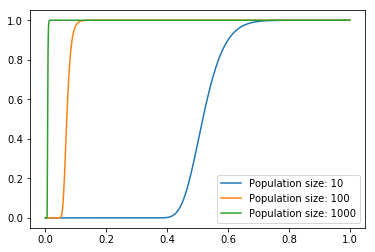
\includegraphics[width=1.5in]{figs/survival_pop_size.png}
%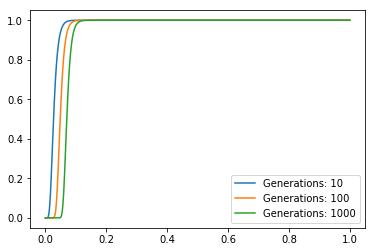
\includegraphics[width=1.5in]{figs/survival_generations.png}
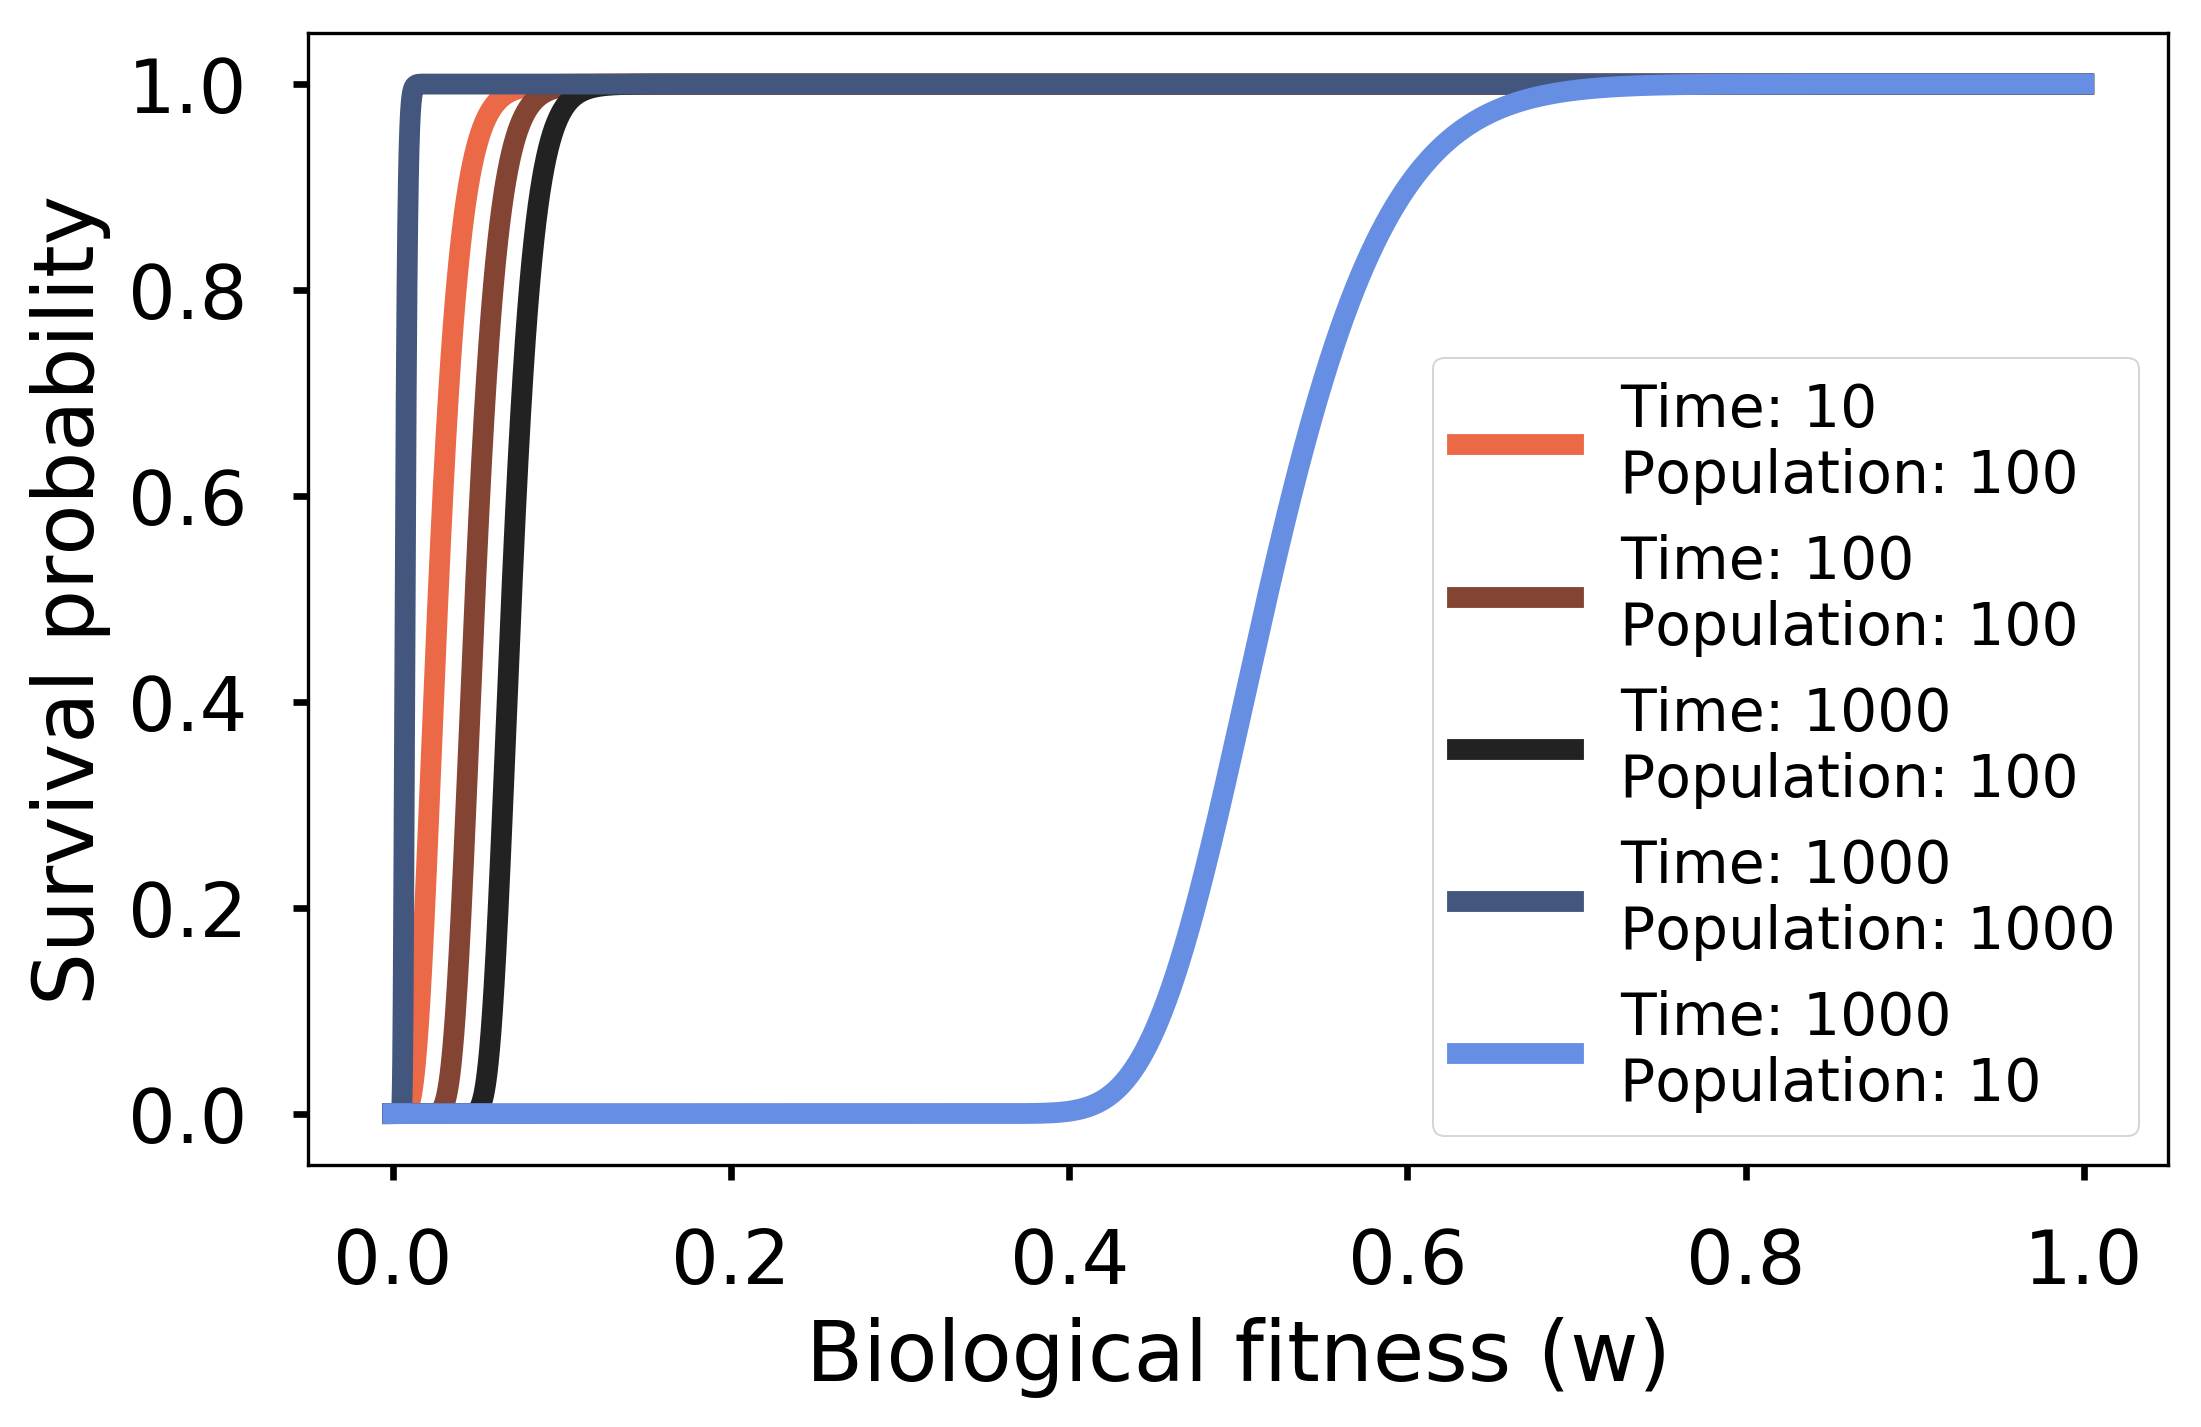
\includegraphics[width=3.4in]{figs/survival.png}
\caption{The probability of long-term survival under lexicase selection across different population sizes and lengths of evolutionary time.}
\label{prob_survival}
\end{figure}

Plotting this function for various parameter values, we see that there is generally a cut-off value where the probability of survival rises abruptly from approximately 0 to approximately 1 (see Figure \ref{prob_survival}). The value at which the transition occurs is effectively the minimal percentage of islands that a genotype must occupy in order to be expected to survive in the long term. This value is closely related to the concept of a minimum viable population in biology, and is useful to consider when making decisions about how large of a population size to use. 

%From this analysis, we can conclude that lexicase selection produces 

%The selection criteria determine which other individuals in the population a given solution is competeing with for space. 

%\subsection{MAP-Elites}

%The criteria for stable coexistence in MAP-Elites are refreshingly straightforward. Like lexicase selection, MAP-Elites can be thought of as an alternative population structure. Each location in the spatial structure can only be occupied by individuals that fall in the correct phenotypic range. Within a location, competitive exclusion happens immediately. Because each individual can only occupy one location in the population, there is no competition. All members of the population have equal biological fitness, $W$, and all are capable of stable coexistence for an infinite length of time (because individuals stay in the population until they are replaced, there isn't even a risk of stochastic extinction).

\subsection{Eco-EA}

Eco-EA is analogous to a traditional resource competition scenario in ecology. All individuals occupy the same region of space, and so they should all compete with each other to the extent that they use the same resources, resulting in more interactions between individuals. For each individual, we can calculate the lowest amount of each resource that can be present in the environment in order for using it to not harm that individual:

\begin{equation}
R^* = \frac{cost}{C_f * score}
\label{eq:ecoea-rstar}
\end{equation}

Where $cost$ is the cost of performing the task, $C_f$ is the fraction of the available resource consumed, and $score$ is how well the individual performed the task (generally normalized to 1). In resource competition theory terms, this value is effectively that individual's $R^*$ for that resource. Note that this definition is subtly different from the definition of $R^*$ traditionally used in ecology, which states that $R^*$ is the lowest value of resource for which a species' per capita population growth is not negative~\cite{chase_ecological_2003}. We frame $R^*$ in terms of benefit rather than population growth, because in evolutionary computation population growth is generally severely restricted by competition for space in the population (alternatively, we could treat space as an additional resource, for which all species compete based on their fitness). Note that a higher $score$ reduces $R^*$, meaning that the individual can benefit from the task even if less of the resource is available, making it a better competitor for that resource. Thus an individual that does the associated task better will be successful even in the presence of many individuals using the resource. A lower $R^*$ has the equivalent meaning in biology.

If individuals use entirely different resources, there will be a high degree of stabilization, meaning they should be able to coexist under a wide range of fitness differences. The more complex coexistence scenario occurs when two individuals compete for the same resources. Ecologists draw a distinction between resources that can be used interchangeably with each other (``substitutable resources'') and resources that can not be used interchangeably (``essential resources''). Resources in Eco-EA are substitutable, because an equivalent fitness gain could be achieved using either (up to a point); one just requires more resource to do so.  In this scenario, two individuals can stably coexist as long as they have lower $R^*$s for opposite resources, and each one consumes more of the resource it has a lower $R^*$ for. Because both $R^*$ and the amount of resource consumed are determined by the individual's score on the task associated with the resource, the latter criterion will always be met. Thus, any pair of individuals for which neither has lower $R^*$ for every resource (i.e. for which neither dominates the other) should be able to coexist, assuming that their fitnesses are similar enough, relative to the intensity of the stabilizing dynamics, which can be calculated based on the resource consumption of each species~\cite{letten_linking_2017}.

Biological fitness, $W$, can be calculated in the same way as in fitness sharing: first, calculate the adjusted fitnesses based on resource use, then use Equation \ref{tournament_equation}. 

\subsection{Summary}

As we would expect based on the fact that they are all billed as diversity maintenance techniques, all of these selection schemes allow for long-term stable coexistence. In the case of fitness sharing and Eco-EA, the criteria are described by Chesson's coexistence theory~\cite{chesson_mechanisms_2000}; each species must limit itself more than it limits others (this requirement is mathematically formalized in Equation \ref{eq:share_coexist_1}). In the case of lexicase selection, the biological fitness (i.e. the percent of ``islands'' the species dominates) must be greater than a cutoff described in Figure \ref{prob_survival}.

Although Eco-EA and fitness sharing have the same coexistence criteria, they have an important difference from each other: in Eco-EA, competition occurs along multiple potentially orthogonal dimensions, whereas in fitness sharing all competition is mediated through a function that summarizes all aspects of an individual. This difference should result in fewer more intense pairwise competitive interaction in Eco-EA than in fitness sharing (although still not as few as in lexicase selection). We predict that these more focused interactions will promote evolutionary divergence. The requirement in Eco-EA that coexisting individuals must be non-dominated suggests that individuals in Eco-EA should fall roughly along a pareto front, similarly to individuals in lexicase selection. An important distinction between these two selection schemes, however, is that lexicase selection's rigid population structure produces strong pressure for generalists, whereas generalists can be successful in Eco-EA.

\section{Empirical Methods}

While theory offers a good mental framework to understand empirical results, it can easily get detached from reality. This issue is exacerbated in the case of systems with substantial stochasticity and feedback loops, such as evolutionary systems. In such situations, the average case predicted by theory may not actually be particularly representative. Thus, to strengthen our intuition for the ecology of these selection schemes, we now investigate them in the context of actual populations. 

\subsection{Interaction networks}
In section 2, we predicted the competitive pressures that different selection schemes exert on a population. We assess the accuracy of these predictions by drawing interaction networks for populations under these selection schemes. For simplicity, we use a population containing 10 vectors of 5 numbers. Each number represents a niche which these individuals are competing to occupy. In fitness sharing, distance is measured as euclidean distance between each pair of vectors. For lexicase selection, each position in the vector is a selection criterion and the individual with the highest value there wins. In Eco-EA, there is a resource associated with each position in the vector and an individual's value at that position defines its ability to use that resource. The fitness landscape is otherwise flat. We compare the same population across all selection schemes. To calculate the effect that a given individual, $A$ has on another individual, $B$, we first calculate the fitness of $A$ in the presence of the whole population. Then we remove $B$ from the population and recalculate the fitness of $A$. The difference between these two fitnesses is the effect of $A$ on $B$. Note that these fitness values are biological fitness, i.e. the probability of being selected to reproduce, rather than the fitness produced by the fitness function.  For fitness sharing and Eco-EA, we assumed a tournament size of 2 when making this calculation.

\subsection{Phylogenetic analysis of evolved populations}
What is the long term effect of these different interaction network topologies? We arrive at a first-order approximation by analyzing the phylogenies of populations evolved under each selection scheme. Across selection schemes, the behavior of a population depends on the part of the fitness landscape that it is currently exploring. If the entire population is climbing a steep hill, all forms of diversity should be low, due to frequent selective sweeps. To asses the effect of such differences in fitness landscapes, we compared phylogenetic diversity across two different genetic programming problems: an easy one and a hard one. The easy task was calculating the square of whatever number was given as input. The hard task was calculating numbers in the Collatz sequence~\cite{helmuth_general_2015}. We evolved linear genetic programs for 1000 generations.We used 11 test cases for the squares problem and 100 test cases for the Collatz problem. Phenotypes were the vectors of inverse error for each test case (so higher scores were better). Fitness was calculated as the sum of these vectors. For lexicase selection and Eco-EA, each test case corresponded to a selection criterion or resource. 

We performed 30 runs of evolution for each selection scheme and each problem. Because of the profound effect of the sharing threshold parameter on the behavior of fitness sharing, we also performed 30 runs each of fitness sharing with five different sharing thresholds. Statistics across selection schemes were calculated using the sharing threshold with the highest phylogentic diversity. For each run, we calculated a variety of metrics, including phenotypic diveristy, genotypic diversity, phylogenetic diversity~\cite{faith_conservation_1992}, and mean pairwise distance of genotypes in the phylogeny~\cite{webb_exploring_2000}. 

\subsection{Statistical methods}
That statistical significance of all comparisons of metrics across conditions was assessed using a Kruskal-Wallis test. Differences between specific conditions were assessed with a post-hoc pairwise Wilcoxon rank-sum test accompanied by a Bonferroni correction for multiple comparisons.

\subsection{Code availability}
Data for the interaction network analysis was generated using a simple simulation written with Python 3.6.3. Graphs were visualized using the networkx package~\cite{hagberg_exploring_2008}. The code for empirical analysis of evolved populations was written in C++ using the [REMOVED FOR DOUBLE-BLIND] library. Statistical analysis was performed using the R statistical computing language version 3.4.3~\cite{r_core_team_r:_2017} and graphs were made with the ggplot2 package~\cite{wickham_ggplot2:_2009}. All code for generating and analyzing the data presented in this paper is open source and available at [REMOVED FOR DOUBLE-BLIND]. 

\section{Results and Discussion}

\subsection{Interaction networks}

\begin{figure}
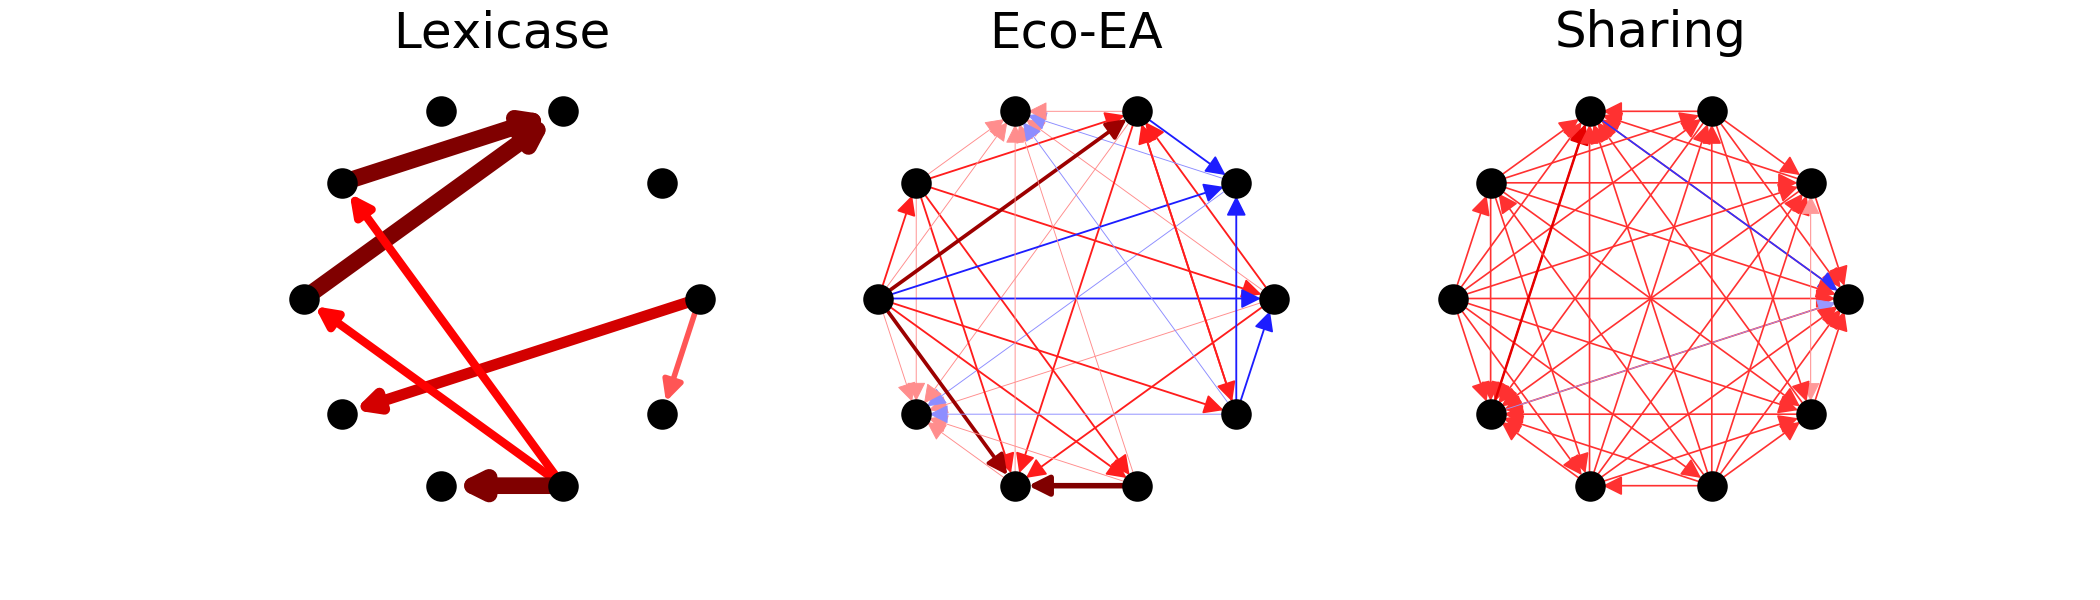
\includegraphics[width=3.5in]{figs/interaction_networks.png}
\caption{Interaction networks for the same community under three different selection schemes: lexicase selection, Eco-EA, and fitness sharing. Red edges indicate harmful interactions, blue edges indicate beneficial interactions. Edge width denotes interaction strength.}
\label{interaction_network}
\end{figure}

There are striking differences among the interaction networks created by the different selection schemes (see Figure~\ref{interaction_network}). Most notably, as we predicted, far fewer individuals interact with each other under lexicase selection, likely due to the rigid population structure governing interactions. Additionally, all of these interactions are negative and acyclic. Eco-EA has far more interactions, presumably due to the fact that organisms are capable of occupying multiple niches at once. A side effect of this increased interconnectedness is that there are also some beneficial interactions; if $A$ competes with $B$ and $B$ competes with $C$, $A$ can help $C$ by suppressing $B$. Although these complex networks of interactions where once believed to produce a chaotic and unstable community [cite that May paper from the 50s], more recent evidence suggests that the presence of many weak interactions can be stabilizing [cite weak interaction effect paper]. Fitness sharing has still more interactions that Eco-EA. These interactions are more equal in strength, and a higher percentage of them are negative. Interestingly, the few positive interactions that do exist are paired with negative interactions in the opposite direction. 


\subsection{Phylogenetic analysis}

\begin{figure}
%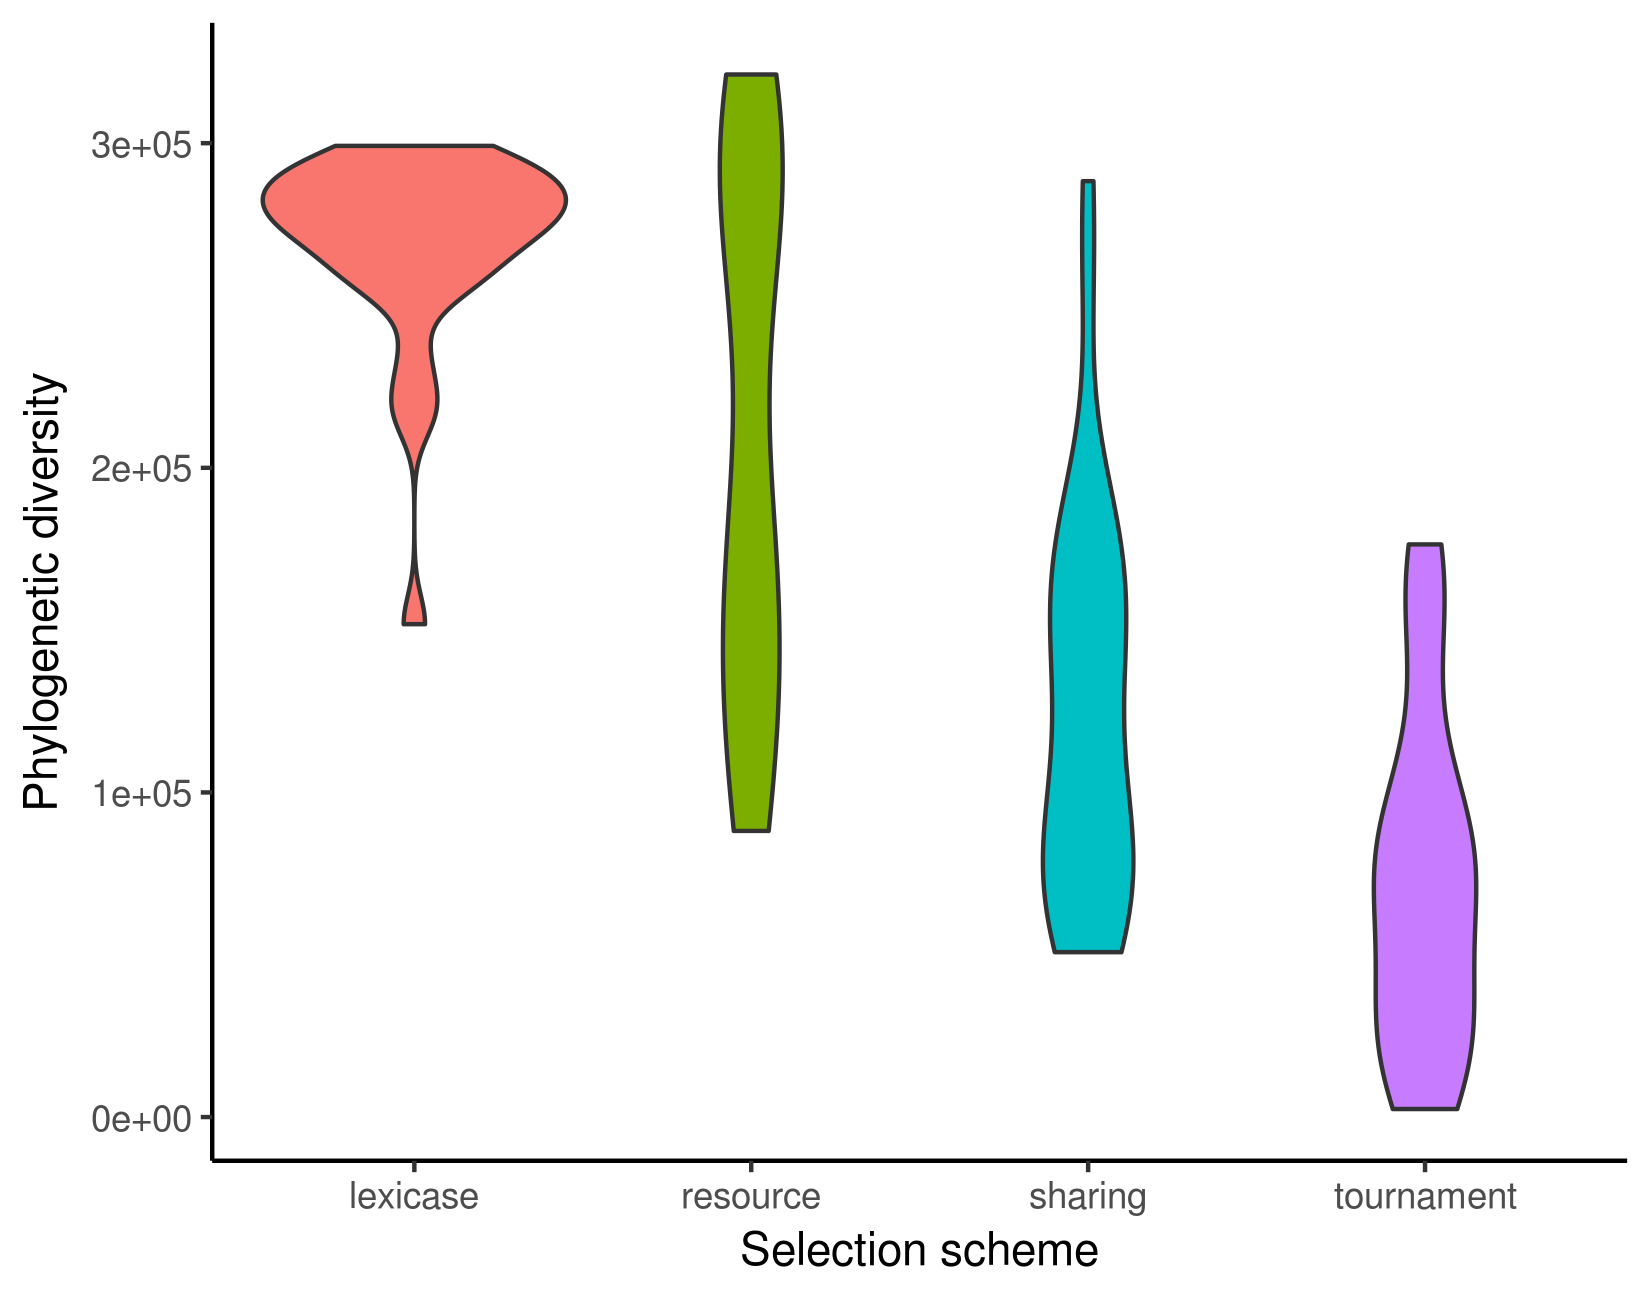
\includegraphics[width=1.6in]{figs/phylo_all.png}
%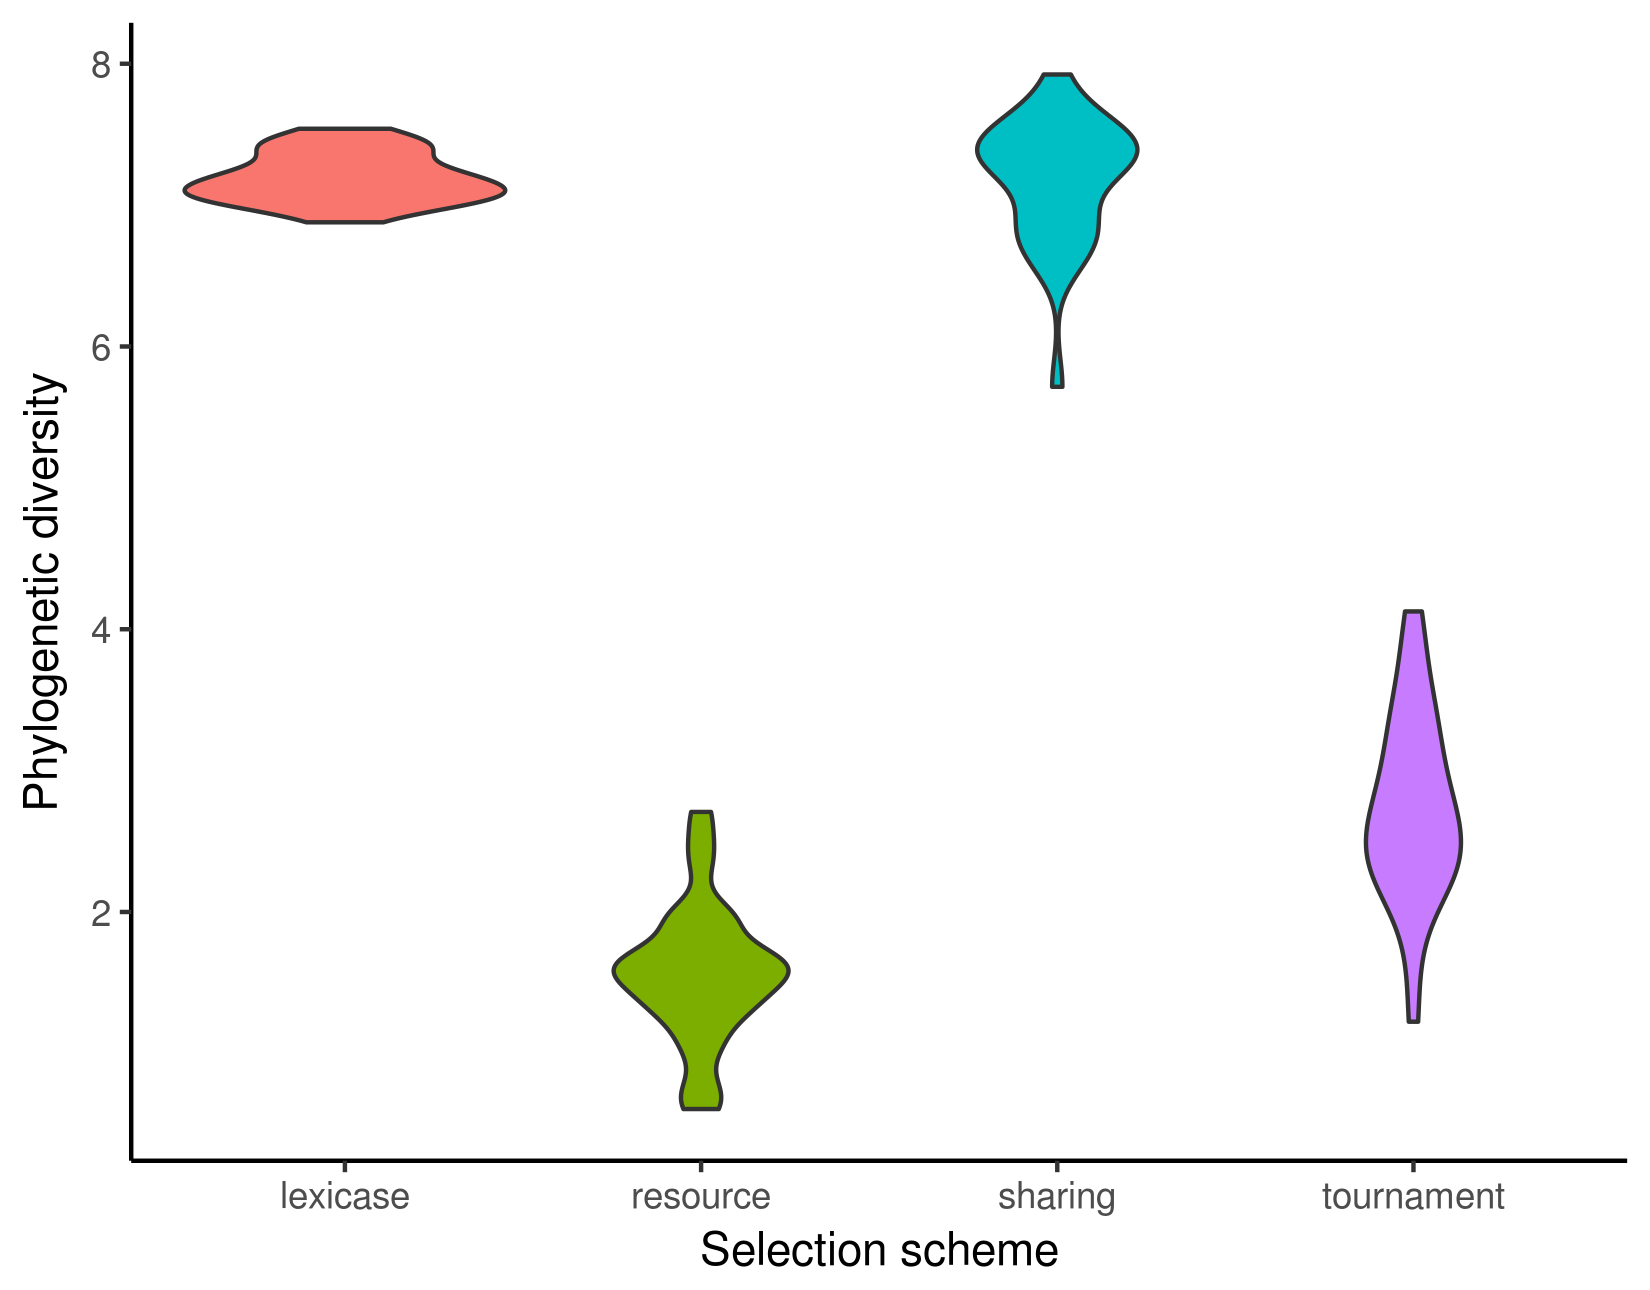
\includegraphics[width=1.6in]{figs/pheno_all.png}
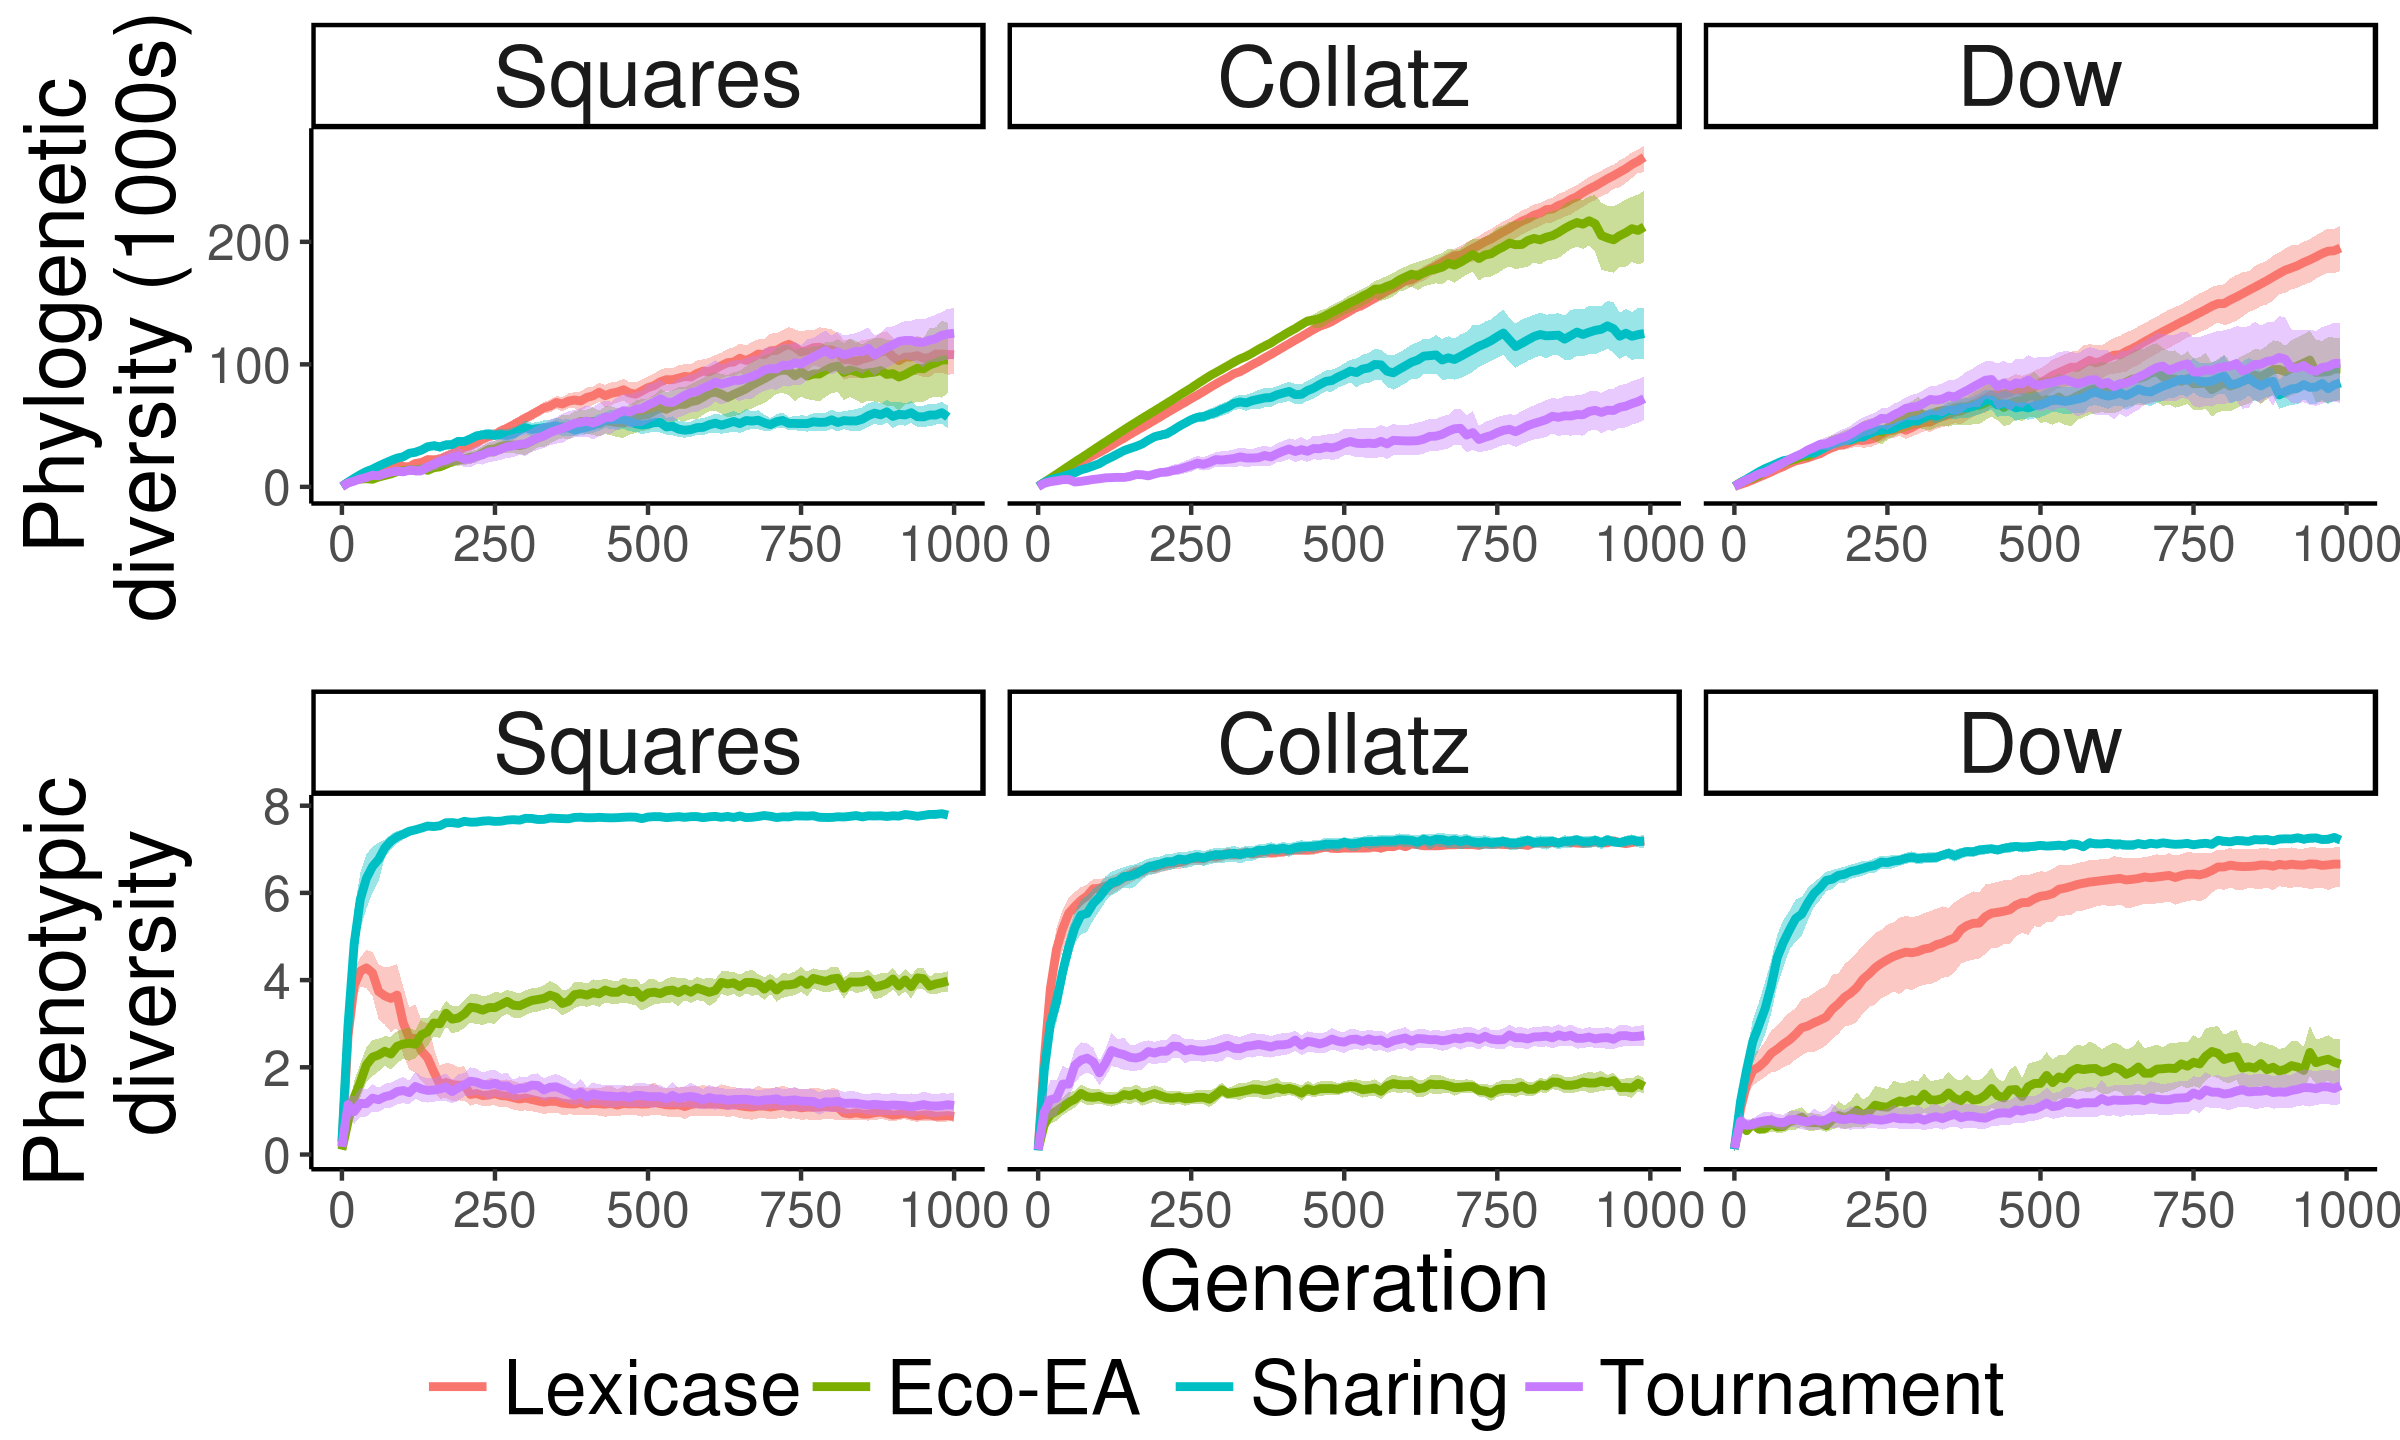
\includegraphics[width=3.4in]{figs/time_all.png}
\caption{Phentypic and phylogenetic diversity over time for each problem. Shaded area is the bootstrapped 95\% confidence interval around the mean.}
\label{phylo_results}
\end{figure}

As hypothesized, phylogenetic diversity is low for all selections schemes on the square problem (see Figure \ref{phylo_results}). This is presumably the result of fitness differences so large that stabilizing effects were insufficient to overcome them. In the context of such a steep evolutionary gradient, such behavior is expected and in many cases desirable. Due to negative frequency dependence, phenotypic diversity remains high for fitness sharing and Eco-EA, even after the point where most populations solved the problem (generally between 200 and 500 generations). For lexicase selection, on the other hand, it initially increases and then drops rapidly as the population converges on the solution.

Results from the Collatz problem support our hypothesis that selection schemes with more restrictions on which individuals compete with which others promote phylogenetic diversity (see Figure \ref{phylo_results}). Lexicase selection and Eco-EA did not have significantly different final phylogenetic diversity (Wilcoxon rank-sum test, p=0.31), but all other pairs of selection schemes did (Wilcoxon rank-sum tests, p $<$ .05). Results for mean pairwise distance were similar, suggesting that lexicase selection and Eco-EA (and to a lesser extent fitness sharing) do promote the coexistence of divergent branches. 

Interestingly, phenotypic diversity does not correlate especially closely with phylogenetic diversity (see Figure \ref{phylo_results}). In particular, Eco-EA has relatively low phenotypic diversity, despite its high phylogenetic diversity. Conversely, fitness sharing has relatively high phenotypic diversity despite its mid-range phylogenetic diversity. This result suggests that whereas lexicase selection and fitness sharing allow similar phenotypes to coexist, Eco-EA forces them to converge. A potential explanation for this difference is that Eco-EA rewards generalists substantially more than lexicase selection.

\begin{figure}
%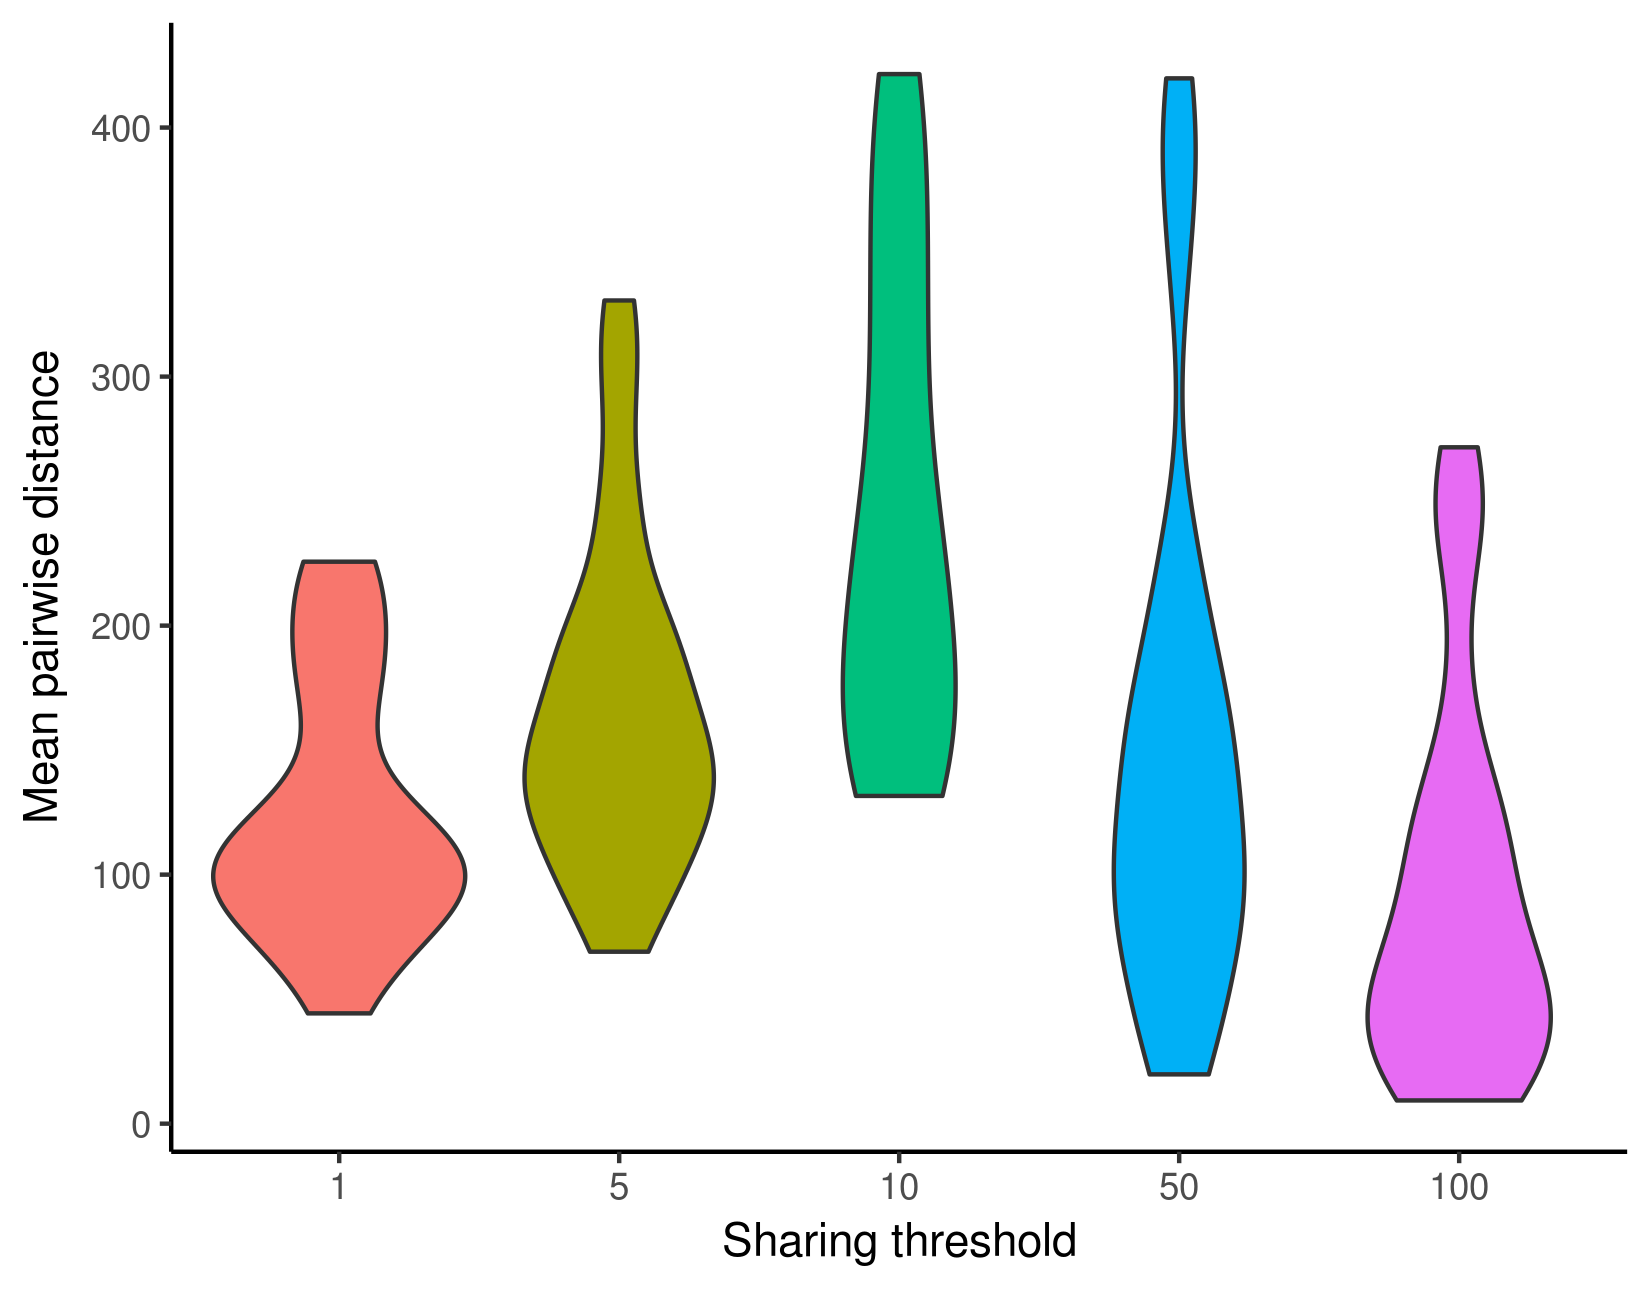
\includegraphics[width=1.6in]{figs/sharing_pairwise_dist.png}
%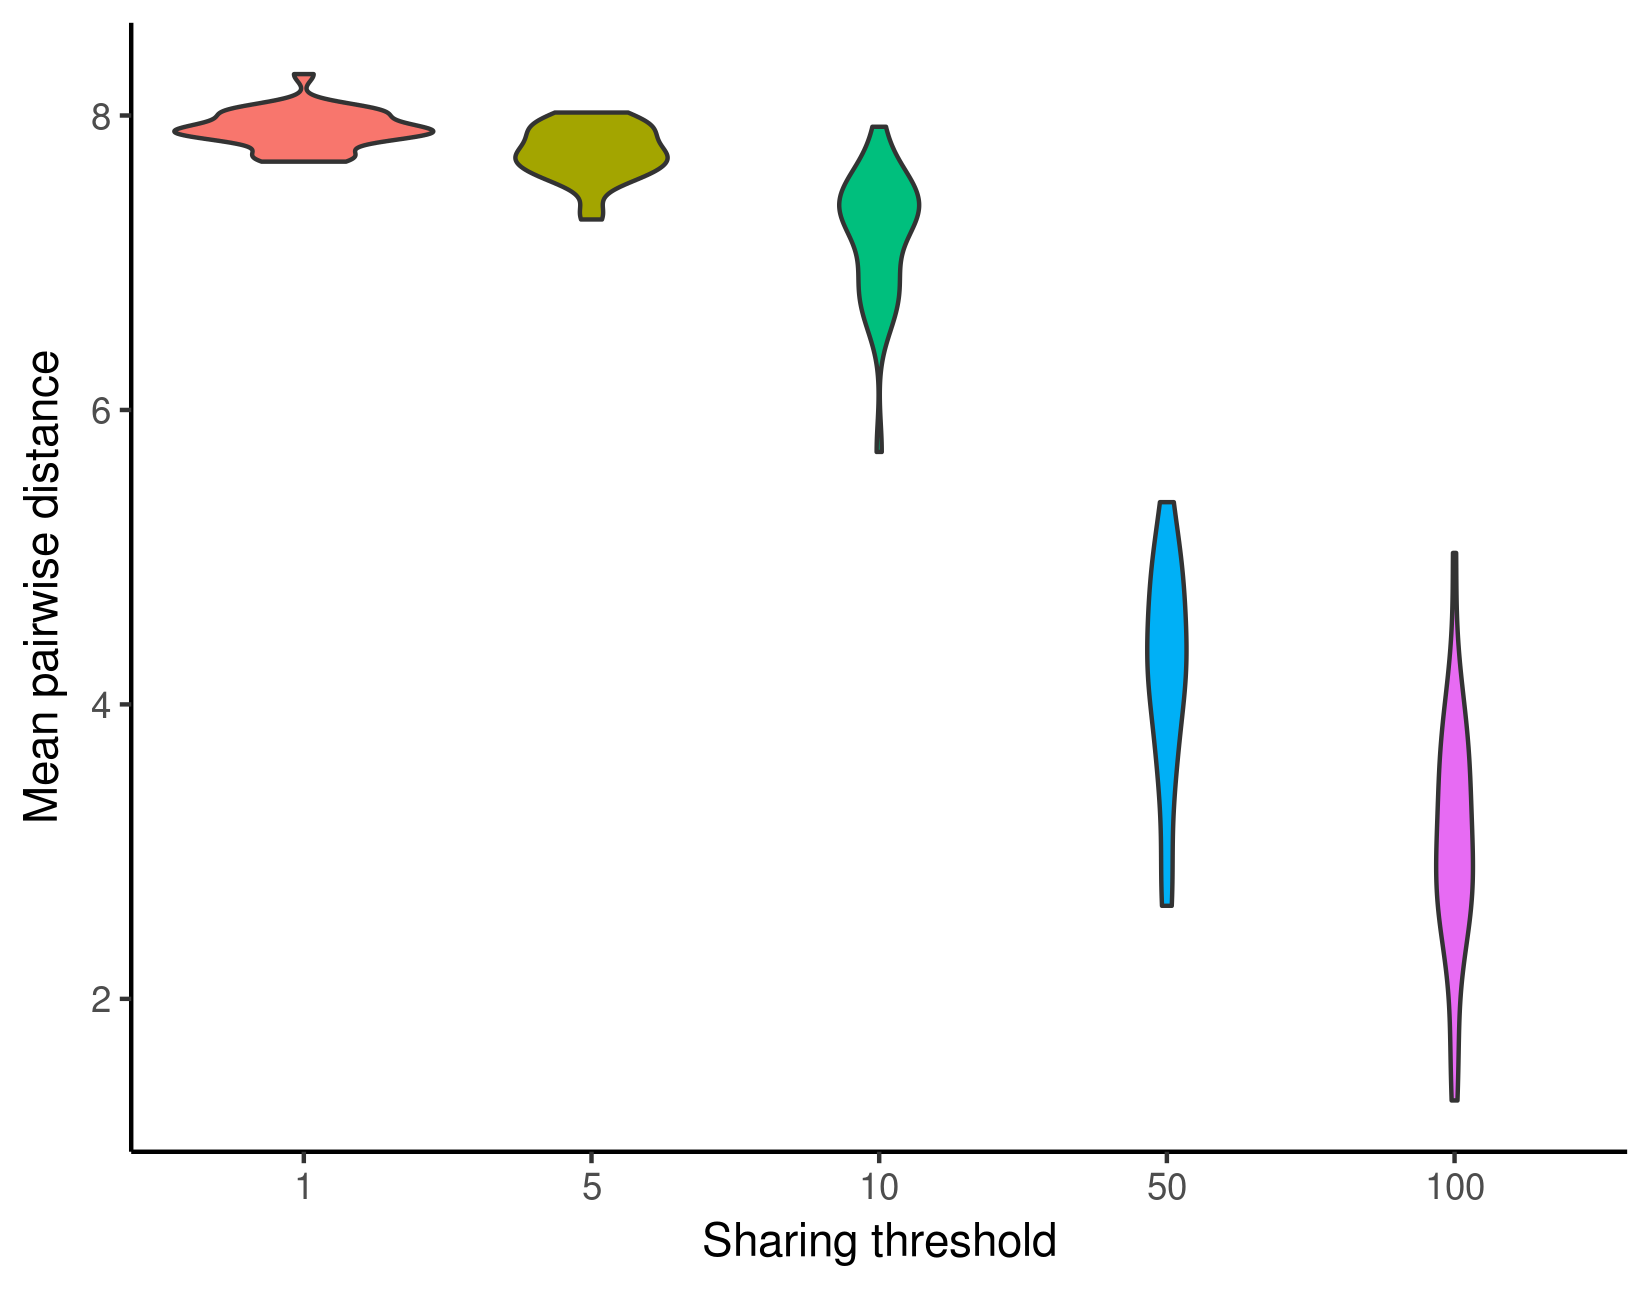
\includegraphics[width=1.6in]{figs/sharing_phenotypic_entropy.png}
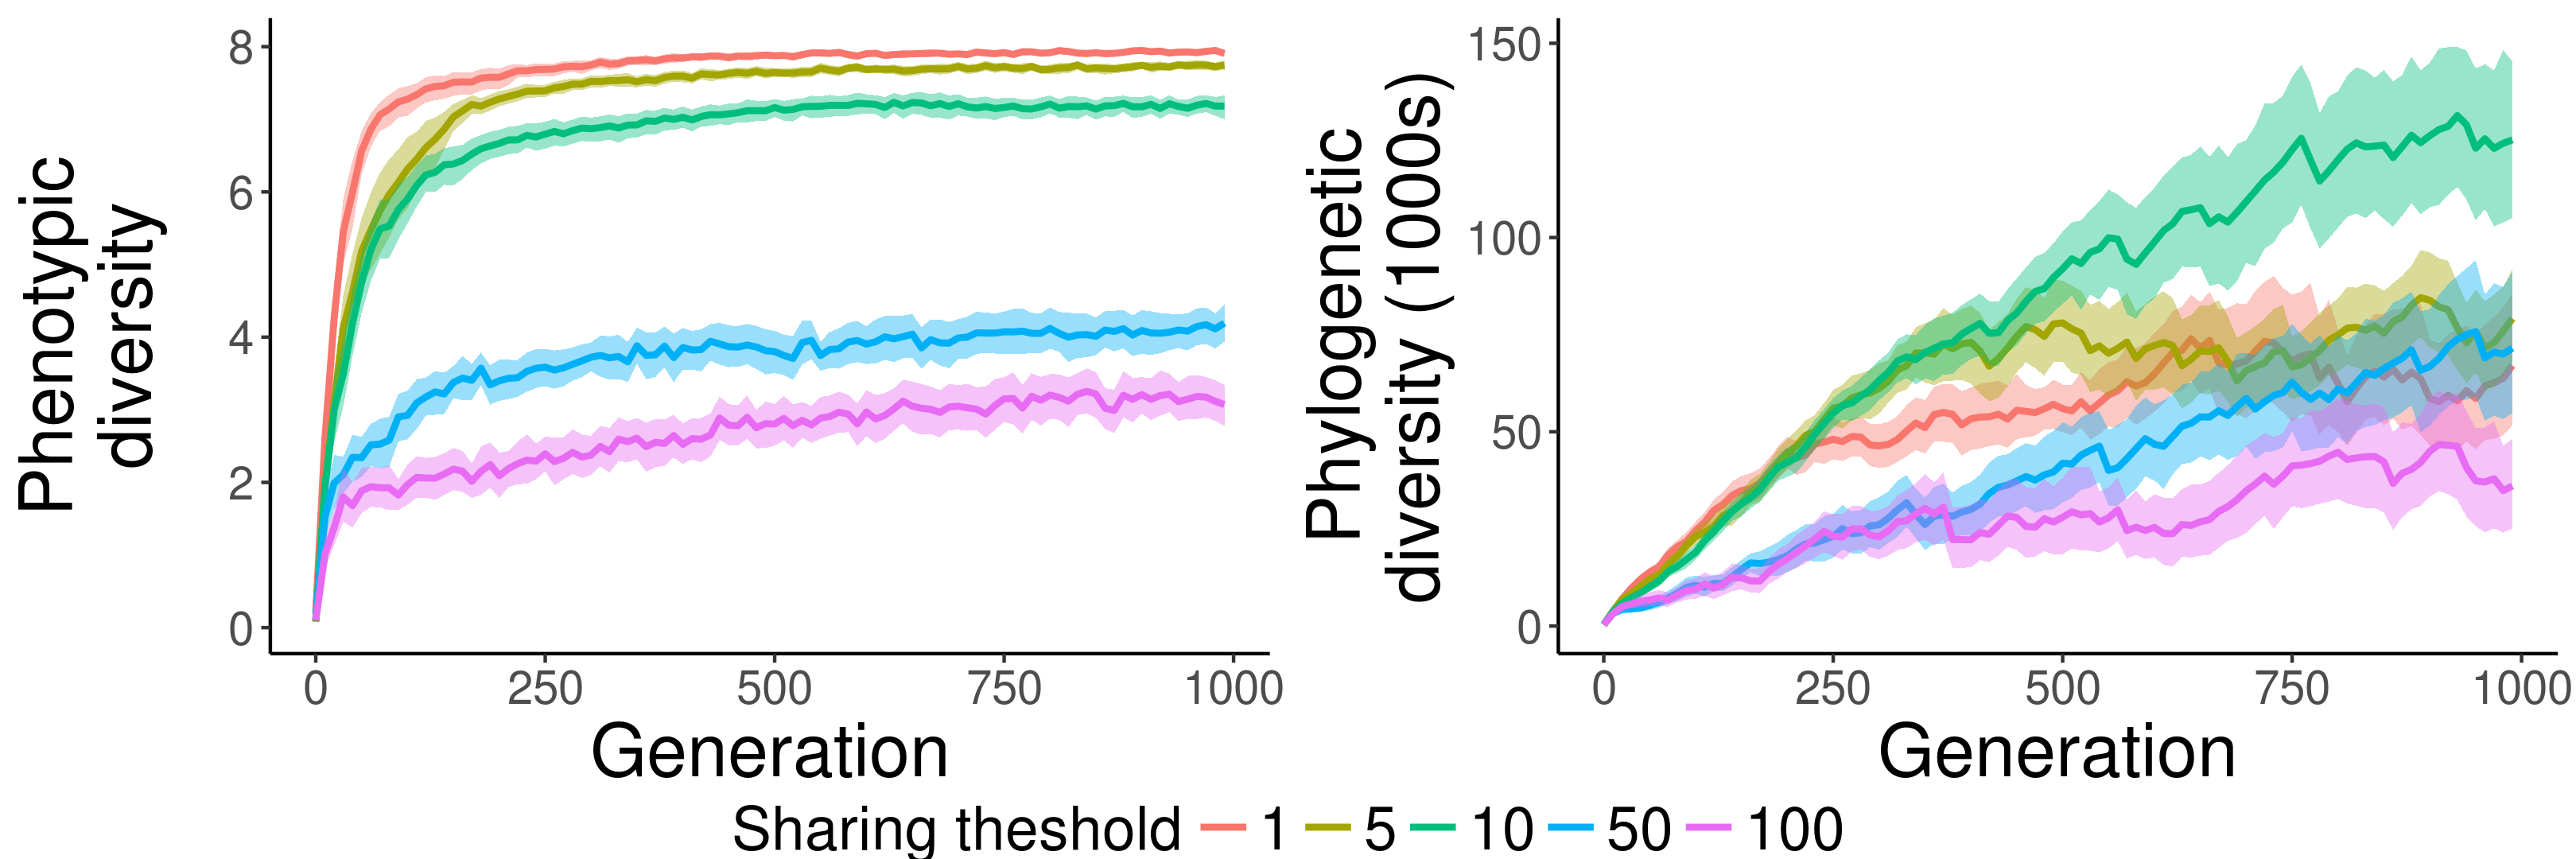
\includegraphics[width=3.4in]{figs/time_sharing.png}
\caption{Phenotypic and phylogenetic diversities across various values of sharing threshold ($\sigma_{\text{share}}$) in the context of the Collatz problem. Shaded area is the bootstrapped 95\% confidence interval around the mean.}
\label{sharing}
\end{figure}

This discrepancy is even more pronounced in the context of selecting a sharing threshold for fitness sharing (see Figure \ref{sharing}). Phenotypic diversity is maximized at a sharing threshold of 1  (Wilcoxon rank-sum tests, p $<$ .05), whereas mean pairwise distance and phylogenetic diversity are highest at a sharing threshold of 10 (Wilcoxon rank-sum tests, p $<$ .05). This result emphasizes the fact that phylogenetic diversity is meaningfully different from phenotypic and genotypic diversity in ways that can affect choice of parameter values.

\section{Conclusions}

In this paper, we have taken a high-level tour of the various tools that ecology can contribute to evolutionary computation. We have used metaphors and mathematical theory from ecology to build up a mental model of the important differences between four different selection schemes. Building on this framework, we empirically measured the interactions between individuals that these different selection schemes create. Finally, we used phylogenetic metrics to explore the long term effects of these selection schemes. Importantly, we have demonstrated that phylogenetic analysis metrics provide insight into the underlying dynamics of diversification above and beyond that provided by genotypic and phenotypic diversity. This result holds across different parameter choices for the same selection scheme, and across different selection schemes, and has implications for choosing which one to use.

From this analysis, we were able to conclude that lexicase selection and Eco-EA promote the evolution and maintenance of solutions that are more evolutionarily distinct. They achieve this result through very different underlying mechanisms. Lexicase selection creates intense competition between a small number of pairs of individuals, whereas Eco-EA creates interactions of a variety of intensity levels across a larger, although still restricted, number of pairs of individuals. As a result, lexicase selection promotes the generation of a large number of specialist phenotypes, while Eco-EA supports a smaller number of more generalist phenotypes. Phenotypes from both selection schemes are expected to fall somewhere along the Pareto front.

Overall, we believe that ecological techniques have much to contribute to our understanding of evolutionary computation, and our work here has barely scratched the surface. In the future, we hope to import more statistical techniques from ecology, and apply them to an even wider range of selection schemes.

\begin{acks}
We thank Alex Lalejini, Matthew Moreno, and Michael Wiser for their helpful comments and suggestions on early drafts of this manuscript. This research has been supported by the National Science Foundation (NSF) BEACON Center under Cooperative Agreement DBI-0939454, by an NSF Graduate Research Fellowship to ED under Grant No. DGE-1424871, and by Michigan State University through computational resources provided by the Institute for Cyber-Enabled Research. Any opinions, findings, and conclusions or recommendations expressed in this material are those of the author(s) and do not necessarily reflect the views of the NSF.
\end{acks}


% \subsection{Citations}
% Citations to articles~\cite{bowman:reasoning,
% clark:pct, braams:babel, herlihy:methodology},
% conference proceedings~\cite{clark:pct} or maybe
% books \cite{Lamport:LaTeX, salas:calculus} listed
% in the Bibliography section of your
% article will occur throughout the text of your article.
% You should use BibTeX to automatically produce this bibliography;
% you simply need to insert one of several citation commands with
% a key of the item cited in the proper location in
% the \texttt{.tex} file~\cite{Lamport:LaTeX}.
% The key is a short reference you invent to uniquely
% identify each work; in this sample document, the key is
% the first author's surname and a
% word from the title.  This identifying key is included
% with each item in the \texttt{.bib} file for your article.

% The details of the construction of the \texttt{.bib} file
% are beyond the scope of this sample document, but more
% information can be found in the \textit{Author's Guide},
% and exhaustive details in the \textit{\LaTeX\ User's
% Guide} by Lamport~\shortcite{Lamport:LaTeX}.

% This article shows only the plainest form
% of the citation command, using \texttt{{\char'134}cite}.

% Some examples.  A paginated journal article \cite{Abril07}, an enumerated
% journal article \cite{Cohen07}, a reference to an entire issue \cite{JCohen96},
% a monograph (whole book) \cite{Kosiur01}, a monograph/whole book in a series (see 2a in spec. document)
% \cite{Harel79}, a divisible-book such as an anthology or compilation \cite{Editor00}
% followed by the same example, however we only output the series if the volume number is given
% \cite{Editor00a} (so Editor00a's series should NOT be present since it has no vol. no.),
% a chapter in a divisible book \cite{Spector90}, a chapter in a divisible book
% in a series \cite{Douglass98}, a multi-volume work as book \cite{Knuth97},
% an article in a proceedings (of a conference, symposium, workshop for example)
% (paginated proceedings article) \cite{Andler79}, a proceedings article
% with all possible elements \cite{Smith10}, an example of an enumerated
% proceedings article \cite{VanGundy07},
% an informally published work \cite{Harel78}, a doctoral dissertation \cite{Clarkson85},
% a master's thesis: \cite{anisi03}, an online document / world wide web
% resource \cite{Thornburg01, Ablamowicz07, Poker06}, a video game (Case 1) \cite{Obama08} and (Case 2) \cite{Novak03}
% and \cite{Lee05} and (Case 3) a patent \cite{JoeScientist001},
% work accepted for publication \cite{rous08}, 'YYYYb'-test for prolific author
% \cite{SaeediMEJ10} and \cite{SaeediJETC10}. Other cites might contain
% 'duplicate' DOI and URLs (some SIAM articles) \cite{Kirschmer:2010:AEI:1958016.1958018}.
% Boris / Barbara Beeton: multi-volume works as books
% \cite{MR781536} and \cite{MR781537}.

% A couple of citations with DOIs: \cite{2004:ITE:1009386.1010128,
%   Kirschmer:2010:AEI:1958016.1958018}. 

% Online citations: \cite{TUGInstmem, Thornburg01, CTANacmart}.  


% \subsection{Tables}
% Because tables cannot be split across pages, the best
% placement for them is typically the top of the page
% nearest their initial cite.  To
% ensure this proper ``floating'' placement of tables, use the
% environment \textbf{table} to enclose the table's contents and
% the table caption.  The contents of the table itself must go
% in the \textbf{tabular} environment, to
% be aligned properly in rows and columns, with the desired
% horizontal and vertical rules.  Again, detailed instructions
% on \textbf{tabular} material
% are found in the \textit{\LaTeX\ User's Guide}.

% Immediately following this sentence is the point at which
% Table~\ref{tab:freq} is included in the input file; compare the
% placement of the table here with the table in the printed
% output of this document.

% \begin{table}
%   \caption{Frequency of Special Characters}
%   \label{tab:freq}
%   \begin{tabular}{ccl}
%     \toprule
%     Non-English or Math&Frequency&Comments\\
%     \midrule
%     \O & 1 in 1,000& For Swedish names\\
%     $\pi$ & 1 in 5& Common in math\\
%     \$ & 4 in 5 & Used in business\\
%     $\Psi^2_1$ & 1 in 40,000& Unexplained usage\\
%   \bottomrule
% \end{tabular}
% \end{table}

% To set a wider table, which takes up the whole width of the page's
% live area, use the environment \textbf{table*} to enclose the table's
% contents and the table caption.  As with a single-column table, this
% wide table will ``float'' to a location deemed more desirable.
% Immediately following this sentence is the point at which
% Table~\ref{tab:commands} is included in the input file; again, it is
% instructive to compare the placement of the table here with the table
% in the printed output of this document.


% \begin{table*}
%   \caption{Some Typical Commands}
%   \label{tab:commands}
%   \begin{tabular}{ccl}
%     \toprule
%     Command &A Number & Comments\\
%     \midrule
%     \texttt{{\char'134}author} & 100& Author \\
%     \texttt{{\char'134}table}& 300 & For tables\\
%     \texttt{{\char'134}table*}& 400& For wider tables\\
%     \bottomrule
%   \end{tabular}
% \end{table*}
% % end the environment with {table*}, NOTE not {table}!

% It is strongly recommended to use the package booktabs~\cite{Fear05}
% and follow its main principles of typography with respect to tables:
% \begin{enumerate}
% \item Never, ever use vertical rules.
% \item Never use double rules.
% \end{enumerate}
% It is also a good idea not to overuse horizontal rules.


% \subsection{Figures}

% Like tables, figures cannot be split across pages; the best placement
% for them is typically the top or the bottom of the page nearest their
% initial cite.  To ensure this proper ``floating'' placement of
% figures, use the environment \textbf{figure} to enclose the figure and
% its caption.

% This sample document contains examples of \texttt{.eps} files to be
% displayable with \LaTeX.  If you work with pdf\LaTeX, use files in the
% \texttt{.pdf} format.  Note that most modern \TeX\ systems will convert
% \texttt{.eps} to \texttt{.pdf} for you on the fly.  More details on
% each of these are found in the \textit{Author's Guide}.

% %\begin{figure}
% %
\includegraphics{fly}
% %\caption{A sample black and white graphic.}
% %\end{figure}

% %\begin{figure}
% %
\includegraphics[height=1in, width=1in]{fly}
% %\caption{A sample black and white graphic
% %that has been resized with the \texttt{includegraphics} command.}
% %\end{figure}


% As was the case with tables, you may want a figure that spans two
% columns.  To do this, and still to ensure proper ``floating''
% placement of tables, use the environment \textbf{figure*} to enclose
% the figure and its caption.  And don't forget to end the environment
% with \textbf{figure*}, not \textbf{figure}!

% %\begin{figure*}
% %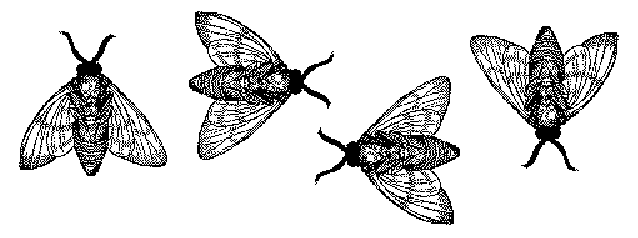
\includegraphics{flies}
% %\caption{A sample black and white graphic
% %that needs to span two columns of text.}
% %\end{figure*}


% %\begin{figure}
% %
\includegraphics[height=1in, width=1in]{rosette}
% %\caption{A sample black and white graphic that has
% %been resized with the \texttt{includegraphics} command.}
% %\end{figure}

% \subsection{Theorem-like Constructs}

% Other common constructs that may occur in your article are the forms
% for logical constructs like theorems, axioms, corollaries and proofs.
% ACM uses two types of these constructs:  theorem-like and
% definition-like.

% Here is a theorem:
% \begin{theorem}
%   Let $W$ be continuous on $[a,b]$.  If $G$ is
%   an antiderivative for $W$ on $[a,b]$, then
%   \begin{displaymath}
%     \int^b_af(t)\,dt = G(b) - G(a).
%   \end{displaymath}
% \end{theorem}

% Here is a definition:
% \begin{definition}
%   If $z$ is irrational, then by $e^z$ we mean the
%   unique number that has
%   logarithm $z$:
%   \begin{displaymath}
%     \log e^z = z.
%   \end{displaymath}
% \end{definition}

% The pre-defined theorem-like constructs are \textbf{theorem},
% \textbf{conjecture}, \textbf{proposition}, \textbf{lemma} and
% \textbf{corollary}.  The pre-defined de\-fi\-ni\-ti\-on-like constructs are
% \textbf{example} and \textbf{definition}.  You can add your own
% constructs using the \textsl{amsthm} interface~\cite{Amsthm15}.  The
% styles used in the \verb|\theoremstyle| command are \textbf{acmplain}
% and \textbf{acmdefinition}.

% Another construct is \textbf{proof}, for example,

% \begin{proof}
%   Suppose on the contrary there exists a real number $L$ such that
%   \begin{displaymath}
%     \lim_{x\rightarrow\infty} \frac{f(x)}{g(x)} = L.
%   \end{displaymath}
%   Then
%   \begin{displaymath}
%     l=\lim_{x\rightarrow c} f(x)
%     = \lim_{x\rightarrow c}
%     \left[ g{x} \cdot \frac{f(x)}{g(x)} \right ]
%     = \lim_{x\rightarrow c} g(x) \cdot \lim_{x\rightarrow c}
%     \frac{f(x)}{g(x)} = 0\cdot L = 0,
%   \end{displaymath}
%   which contradicts our assumption that $l\neq 0$.
% \end{proof}

% \section{Conclusions}
% This paragraph will end the body of this sample document.
% Remember that you might still have Acknowledgments or
% Appendices; brief samples of these
% follow.  There is still the Bibliography to deal with; and
% we will make a disclaimer about that here: with the exception
% of the reference to the \LaTeX\ book, the citations in
% this paper are to articles which have nothing to
% do with the present subject and are used as
% examples only.
% %\end{document}  % This is where a 'short' article might terminate



% \appendix
% %Appendix A
% \section{Headings in Appendices}
% The rules about hierarchical headings discussed above for
% the body of the article are different in the appendices.
% In the \textbf{appendix} environment, the command
% \textbf{section} is used to
% indicate the start of each Appendix, with alphabetic order
% designation (i.e., the first is A, the second B, etc.) and
% a title (if you include one).  So, if you need
% hierarchical structure
% \textit{within} an Appendix, start with \textbf{subsection} as the
% highest level. Here is an outline of the body of this
% document in Appendix-appropriate form:
% \subsection{Introduction}
% \subsection{The Body of the Paper}
% \subsubsection{Type Changes and  Special Characters}
% \subsubsection{Math Equations}
% \paragraph{Inline (In-text) Equations}
% \paragraph{Display Equations}
% \subsubsection{Citations}
% \subsubsection{Tables}
% \subsubsection{Figures}
% \subsubsection{Theorem-like Constructs}
% \subsubsection*{A Caveat for the \TeX\ Expert}
% \subsection{Conclusions}
% \subsection{References}
% Generated by bibtex from your \texttt{.bib} file.  Run latex,
% then bibtex, then latex twice (to resolve references)
% to create the \texttt{.bbl} file.  Insert that \texttt{.bbl}
% file into the \texttt{.tex} source file and comment out
% the command \texttt{{\char'134}thebibliography}.
% % This next section command marks the start of
% % Appendix B, and does not continue the present hierarchy
% \section{More Help for the Hardy}

% Of course, reading the source code is always useful.  The file
% \path{acmart.pdf} contains both the user guide and the commented
% code.

